\documentclass{article}
\usepackage{multicol}
\usepackage{float}
\setlength{\columnsep}{1cm}

\usepackage{breakcites} % break citations so they don't spill over margin
% Center the section headers
\usepackage{sectsty}
% \usepackage{titlesec}
\usepackage{lipsum}
\sectionfont{\centering} % center just the titles

% margin adjustment
\usepackage[a4paper,right=26mm,left=26mm,top=26mm,bottom=26mm]{geometry} % https://www.sharelatex.com/blog/2013/08/06/thesis-series-pt2.html

% inserting title page
\usepackage{pdfpages}

\usepackage[english]{babel}
\usepackage{inputenc}

 % insert clickable references and urls
\usepackage{url}
\usepackage{hyperref}
\graphicspath{ {images/final/} } % image path

\usepackage[nottoc]{tocbibind}

% Latex commands / macros
    \newcommand{\mat}[2][ccccccccccccccccccccccccccccccccccccccccccccc]
	    {\left[ \arraycolsep=4pt\def\arraystretch{1.5}
				\begin{array}{#1} #2 \\ 
				\end{array} 
		\right]}

	\newcommand{\crossmat}[1]{\mat{#1{^\times}}}

	\newcommand{\pvec}[1]{\vec{#1}\mkern2mu\vphantom{#1}}
    \newcommand{\mse}{\textrm{MSE}}

    % Position vector macros
    \newcommand{\prpr}{\pvec{p}'_s} % position of the tool sphere (display)
    \newcommand{\ps}{\pvec{p}_s} % position of the tool rear (inertial)

    \newcommand{\prpr}{\pvec{p}'_r} % position of the tool rear (display)
    \newcommand{\pr}{\pvec{p}_r} % position of the tool rear (inertial)
    \newcommand{\pre}{\hat{\pvec{p}}_r}

    \newcommand{\pfpr}{\pvec{p}'_f}
    \newcommand{\pf}{\pvec{p}_f}
    \newcommand{\pfe}{\hat{\pvec{p}}_f}

    \newcommand{\pc}{\pvec{p}_c}
    \newcommand{\pd}{\pvec{p}_d}

    \newcommand{\pu}{\pvec{p}_u}

    % Attitude macros
    \newcommand{\A}{\mathbf{A}} % attitude of the display
    \newcommand{\Ad}{\mathbf{A}_d} % attitude of the display
    \newcommand{\Ac}{\mathbf{A}_c} % attitude of the camera
    \newcommand{\At}{\mathbf{A}_t} % attitude of the tool
    \newcommand{\Atpr}{\mathbf{A}'_t} % attitude of the tool

    \newcommand{\Adinv}{\mathbf{A}^{-1}_d} % attitude of the display
    \newcommand{\Acinv}{\mathbf{A}^{-1}_c} % attitude of the camera
    \newcommand{\Atinv}{\mathbf{A}^{-1}_t} % attitude of the tool

    % Quaternion macros
	\newcommand{\q}{\overline{\mathbf{q}}}
    \newcommand{\qk}{\overline{\mathbf{q}}_k}
    \newcommand{\qkp}{\overline{\mathbf{q}}_k^{-}}
    \newcommand{\qke}{\overline{\mathbf{q}}_k^{-}}
	\newcommand{\qc}{\q_c}
	\newcommand{\qd}{\q_d}
	\newcommand{\qt}{\q_t}

    % Error quaternions
	\newcommand{\dq}{\delta\q_t}
	\newcommand{\dqw}{\delta q_4}
    \newcommand{\dqvec}{\delta \vec{q}}

    \newcommand{\dt}{\delta\theta}
    \newcommand{\dtvec}{\delta\vec{\theta}}

	% Covariance matrix macros
    \newcommand{\cov}{\mathbf{\Sigma}}

    % Quaternion error covariances
	\newcommand{\Pqc}{\mathbf{\Sigma}_{qc}}
	\newcommand{\Pqd}{\mathbf{\Sigma}_{qd}}
	\newcommand{\Pqt}{\mathbf{\Sigma}_{qt}}

    % Angular error covariances
	\newcommand{\Ptc}{\mathbf{\Sigma}_{\theta c}}
	\newcommand{\Ptd}{\mathbf{\Sigma}_{\theta d}}
	\newcommand{\Ptt}{\mathbf{\Sigma}_{\theta t}}

	\newcommand{\Pacpr}{\mathbf{\Sigma}'_{ac}}
	\newcommand{\Padpr}{\mathbf{\Sigma}'_{ad}}
	\newcommand{\Patpr}{\mathbf{\Sigma}'_{at}}

	\newcommand{\Pps}{\mathbf{\Sigma}_{ps}}
	\newcommand{\Ppr}{\mathbf{\Sigma}_{pr}}
	\newcommand{\Ppf}{\mathbf{\Sigma}_{pf}}
	\newcommand{\Ppc}{\mathbf{\Sigma}_{pc}}
	\newcommand{\Ppd}{\mathbf{\Sigma}_{pd}}
    \newcommand{\Ppl}{\mathbf{\Sigma}_{l}}

	\newcommand{\Pprpr}{\mathbf{\Sigma}'_{ps}}
	\newcommand{\Pprpr}{\mathbf{\Sigma}'_{pr}}
	\newcommand{\Ppfpr}{\mathbf{\Sigma}'_{pf}}

    % predicted covariance
    \newcommand{\Ppp}{\mathbf{P}_{k}^{-}}

	% Tool length macro
	\newcommand{\pl}{\vec{p}_l}
    \newcommand{\ple}{\hat{\vec{p}}_l}
    \newcommand{\plpr}{\pvec{p}'_l}

	% Section header commands
    \renewcommand{\thesection}{\Roman{section}.} 
    \renewcommand{\thesubsection}{\Alph{subsection}.}
    \renewcommand{\thesubsubsection}{\thesubsection\arabic{subsubsection}}

	% Miscelanous macros
	\newcommand{\tab}{ \textrm{ \ \ \ \ } }

    \newcommand{\z}{\mathbf{\vec{z}}}
    \newcommand{\y}{\mathbf{\vec{y}}}
    \newcommand{\x}{\mathbf{\vec{x}}}

    % Object tracking commands
    \newcommand{\xd}{\dot{x}}
    \newcommand{\xdd}{\ddot{x}}

    % Gyro input
    \newcommand{\gyro}{\vec{\omega}}

    \newcommand{\degtwo}{^{\circ} }
    \newcommand{\Hz}{\textrm{Hz}}

    \newcommand{\deldq}{\frac{\partial \pl}{\partial \dqvec} }
    \newcommand{\ddq}{\frac{\partial}{\partial \dqvec} }

    \newcommand{\tr}{\textrm{tr}}



%%%%%%%%%%%%%%%%%%%%%%%%%%%%%%%%%%%%%%%%%%%%%%%%%%%%%%%%%%%%%%%%%%%%%%%%%%%%%%%
%% TITLE PAGE and contents
%%%%%%%%%%%%%%%%%%%%%%%%%%%%%%%%%%%%%%%%%%%%%%%%%%%%%%%%%%%%%%%%%%%%%%%%%%%%%%%

\begin{document}
\includepdf{title}
\tableofcontents
\listoffigures


%%%%%%%%%%%%%%%%%%%%%%%%%%%%%%%%%%%%%%%%%%%%%%%%%%%%%%%%%%%%%%%%%%%%%%%%%%%%%%%
%% Abstract
%%%%%%%%%%%%%%%%%%%%%%%%%%%%%%%%%%%%%%%%%%%%%%%%%%%%%%%%%%%%%%%%%%%%%%%%%%%%%%%

\section{Abstract}
The 3D Interaction Tool is a hand-held device that enables a user to interact with virtual reality applications. Since both the position and orientation of the tool are tracked, user input with the tool accomplishes tasks such as selecting, translating, and rotating three-dimensional objects, or free-hand drawing in space. The tool�s position is tracked by a software application that filters observations from a camera attached to the virtual reality display, and the orientation is found by means of observations from an inertial measurement unit attached to the tool itself. Simple computer-aided design and drawing applications are possible with the capabilities of the 3D Interaction Tool. 

\begin{flushleft}

\section{Nomenclature}

% Position vector definitions
\textbf{Position vectors definitions in the inertial coordinate frame}: \\
$ \pr \equiv $ position of the tool rear \\
$ \pf \equiv $ position of the tool front \\
$ \pl \equiv $ span vector that connects in the rear of the tool to the front of the tool \\
$ \pc \equiv $ position of the tracking camera \\
$ \pd \equiv $ position of the virtual reality display \\

\medskip

% Rotated position vector definitions
\textbf{Rotated position vectors}: \\
$ \prpr \equiv $ position of the tool rear in display coordinates \\
$ \pfpr \equiv $ position of the tool front in display coordinates \\
$ \plpr \equiv $ span vector in the body coordinate system of the interaction tool \\

\medskip

% Attitude matrix definitions
\textbf{Attitude matrices}: \\
$ \Ac \equiv $ attitude of the tracking camera \\
$ \Ad \equiv $ attitude of the virtual reality display \\
$ \At \equiv $ attitude of the interaction tool \\
$ \Atpr \equiv $ attitude of the interaction tool in display coordinates \\

\medskip

% Quaternion definitions
% $ \qd \equiv $ attitude of the virtual reality display \\
\textbf{Body-referenced quaternion representations of attitude}: \\
$ \qc \equiv $ attitude of the tracking camera \\
$ \qt \equiv $ attitude of the interaction tool \\

\medskip

% Covariance definitions
\textbf{Position error covariances in inertial coordinate frame}: \\
$ \Ppr \equiv $ covariance of the position of the rear of the interaction tool\\
$ \Ppf \equiv $ covariance of the position of the front of the interaction tool\\
% $ \Ppc \equiv $ covariance of the position of the tracking camera \\
% $ \Ppd \equiv $ covariance of the position of the virtual reality display \\

\medskip

% \textbf{Attitude error covariances in the inertial coordinate frame}: \\
% $ \Pqc \equiv $ covariance of the tracking camera attitude quaternion error \\
% $ \Pqd \equiv $ covariance of the display attitude quaternion error \\
% $ \Pqt \equiv $ covariance of the interaction tool attitude quaternion error \\

\medskip

\textbf{Position error covariances in rotated body coordinates}: \\
% $ \Pprpr \equiv $ covariance of the sphereical tracking target position \\
$ \Pprpr \equiv $ covariance of the position of the rear of the interaction tool in rotated coordinates\\
$ \Ppfpr \equiv $ covariance of the position of the front of the interaction tool in rotated coordinates\\

\medskip

\textbf{General}: \\
$\q \equiv $ quaternion  \\
$A(\q) \equiv $ rotation matrix from the world coordinate frame to the orientation specified by \q \\
$\dq \equiv $ small orientation errors in the quaternion \\
$\dt \equiv $ small orientation errors \\

\medskip

\textbf{Kalman Filter}
$Q \equiv $ process noise matrix of the Kalman filter
$R \equiv $ measurement noise matrix of the Kalman filter
$K \equiv $ Kalman gain
$H \equiv $ measurement sensitivity matrix
$\mu \equiv $ innovation
% $ \Pprpr \equiv $ covariance of the sphereical tracking target position \\
% \textbf{Attitude error covariances in the rotated body coordinates}: \\
% $ \Pacpr \equiv $ covariance of the tracking camera attitude angular error \\
% $ \Padpr \equiv $ covariance of the display attitude angular error \\
% $ \Patpr \equiv $ covariance of the interaction tool attitude angular error \\

%%%%%%%%%%%%%%%%%%%%%%%%%%%%%%%%%%%%%%%%%%%%%%%%%%%%%%%%%%%%%%%%%%%%%%%%%%%%%%%
%% INTRODUCTION
%%%%%%%%%%%%%%%%%%%%%%%%%%%%%%%%%%%%%%%%%%%%%%%%%%%%%%%%%%%%%%%%%%%%%%%%%%%%%%%

\section{Introduction}

\subsection{Motivation}

As much as \$25 billion could be spent on virtual reality (VR) and augmented reality (AR) software applications by 2025 \cite{Bloomberg-01-13}. There are two primary modes of user-input that are possible for these applications: indirect and direct. Indirect input devices translate the user's physical movements into the motion of a virtual cursor by means of a fixed transformation. Common examples of indirect input devices are a mouse or joystick. Direct input devices also translate physical to virtual movements, but this transformation is one-to-one. For example, a touch screen is a direct input device because the physical location of the user's press is collocated with the virtual click. 

\medskip

With the advent of virtual reality applications the following question must be answered: which of these input paradigms -- indirect or direct -- will prove most useful for interacting with virtual reality applications? While indirect input devices have achieved widespread popularity for two-dimensional displays, the direct input paradigm for VR applications embraces the immersion of a user in a VR experience. Direct input devices allow users to reach out and interact with the objects of their virtual space, just as they would with objects in their physical space. 

\subsection{Design Approach}

The 3D Interaction Tool is a novel, low-cost 3D input device. In particular, the tool is well-suited for VR applications that use a mobile-phone for the virtual reality display, such as for those applications that run on the Google Cardboard or other low cost solutions. This versatility of the 3D Interaction Tool comes from the simple requirement that the VR display have a front-facing camera attached. This makes the tracking system compatible with any smartphone. The purpose of the 3D Interaction Tool is to demonstrate the functionality of this versatile tracking system. While the tool itself is designed for use with a tracking system on a VR display, the scope of this report is to evaluate the tool's performance in a more controlled environment. The simplifying assumptions necessary to do this are specified below. 

\section{Background}

\subsection{Commercial Solutions}

Recent market trends suggest that direct input devices are on the rise for consumers. Two of these direct input devices, the Oculus Touch controller and the HTC Valve controller are achieving widespread publicity surrounding the commercial release of virtual reality headsets \cite{ValveControllers} \cite{OculusTouch1} \cite{OculusTouch2}. These two controllers are shown in Figure \ref{fig:vrcontrollers}, with the Oculus Touch depicted on the left and the HTC Controllers depicted on the right. While originally scheduled for release alongside the Oculus VR headset at the end of March 2016, the Oculus Touch controller will be available in the second half of 2016 \cite{OculusTouchDelay}. Meanwhile the Valve controllers have been reviewed in preparation for the release of the HTC Vive headset at the beginning of April, 2016, and their utility has been demonstrated with a three-dimensional sketching program by Google called TiltBrush \cite{TiltBruth}. These input devices track both their position and orientation, making them degree-of-freedom (6DOF) controllers. While the 6DOF controllers are reported to work well with their respective headsets, the headsets are expensive -- both retail for more than \$600 -- and the controllers are not useful with other VR displays. Thus, two of the drawbacks of these commercial VR controllers are their cost and their compatibility requirements. 

\begin{figure}[H]
    \begin{center}$
        \begin{array}{cc}
            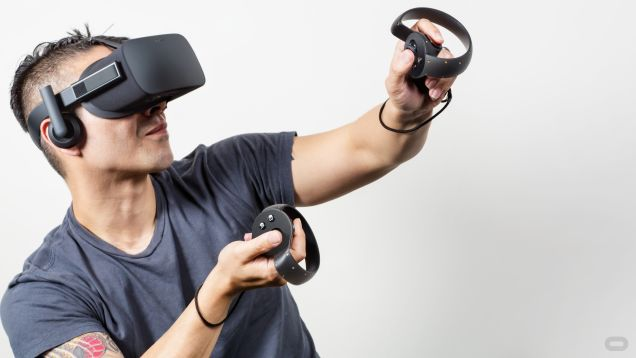
\includegraphics[width=0.5\textwidth]{OculusTouch} &  
            \includegraphics[width=0.5\textwidth]{HtcController}
        \end{array}$
    \end{center}
    \caption{Commercial VR input devices}
    \label{fig:vrcontrollers}
\end{figure}



\subsection{3D Interaction Techniques and their Applications}

Three-dimensional interaction techniques can be separated into several categories. First, there are interactions that manipulate objects. These interactions accomplish tasks such as rotating, translating, or scaling three dimensional objects. Second, there are interactions that manipulate 3D viewpoint, allowing the user to adjust their field of view. Lastly, there are interactions that control an application. Application control interactions include navigating menus or widgets associated with the application logic. The first set of tasks, those that manipulate objects, have largely been the focus of three-dimensional input device design \cite{hand1997}, and the 3D Interaction Tool is designed the object manipulation tasks in mind.

\medskip

Object manipulation tasks are required in artistic and design applications. Several projects have demonstrated the usefulness of 3D input techniques to perform these tasks. For example, the HoloSketch project demonstrated a 3D wand for object creation and manipulation. In HoloSketch the wand could be used for drawing and animating three dimensional objects in a virtual reality environement (VE) \cite{deering1995}. The HoloSketch wand also enabled a user to create free-hand drawings in three-space. 

\medskip

The CavePainting research also allowed a user to manipulate objects using an input device -- and not just one but many such input devices, such as paint brushes and paint buckets. These physical props were used to create artistic works in VE \cite{keefe2001}. The props gave users a very tactile experience of virtual object manipulation, and the tracking system, known as the Cave, was able to track these objects while the user walked around in the virtual environment. Both of these solutions investigated the 3D input device interface for the process of artistic creation. 

\medskip

In addition to artistic applications, 3D interface design has been explored for its potential use for CAD applications. For example, the 6D hands project enabled a user to interact with objects in a 3D modelling environment to more quickly and efficiently perform object manipulation tasks \cite{wang2011}.

\subsection{Tracking Systems for 3D Input Devices}

The methods of tracking objects in virtual environments are numerous \cite{rolland2001}. These tracking methods are a subset of six degree of freedom tracking approaches, and none of these tracking systems are without drawbacks, leading researchers to develop tracking systems that are well-suited to the needs of their particular application \cite{ribo2001}. The main categories of 6DOF trackers for virtual environments are mechanical, inertial, acoustic, magnetic, and optical \cite{welch2002}.

\section{Design Goals}

There are two broad approaches to 3D input device design. First, there are approaches focused on designing the user-interface for the device. This user-interface would be suitable for a particular application. In short, this approach attempts to answer the question: will this device be usable? Second, there are approaches that explore the functionality of the device for a number of different types of applications, asking the question: will this device be high performance? This report seeks to answer this second question for a three-dimensional input device tracked with a particular configuration of a 6DOF tracking system. 

\subsection{Usability}


The usability requirements presented in Figure \ref{fig:usability} must be met for the tool to succeed as an \textit{input} device for VR software applications. 

\begin{figure}[H]
	\begin{center}
		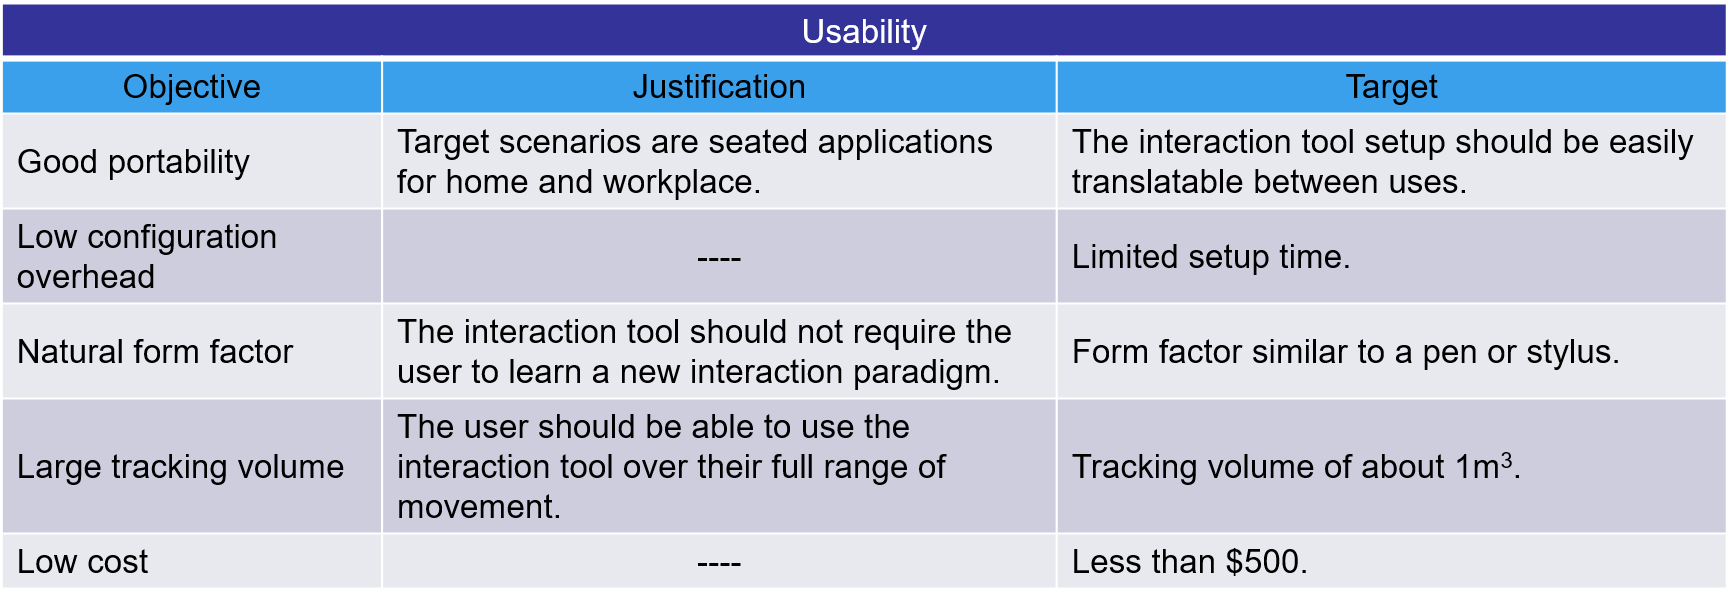
\includegraphics[width=0.8\textwidth]{Usability}
	\end{center}
	\caption{Usability design objectives}
	\label{fig:usability}
\end{figure}

The first of these criteria is portability. The user should be able to use the input device wherever they are using a virtual reality display, without having to precalibrate their environment. Note that this portability objective is different from a \textit{mobility} objective. Mobility would allow unrestricted movement of the device. The reason portability is chosen as a design requirement rather than mobility is that low-cost virtual reality displays such as Google Cardboard are extremely portable and not very mobile. When a smartphone is used as a virtual reality display, it is not aware of its position in its environment. This is true of other low-cost virtual reality displays as well, such as the Samsung GearVR \cite{gearvr}. Thus, the device is chosen to be as portable as the displays with which it would be used. 

\medskip

The second usability design objective is a natural form factor for the device. The natural form factor serves the ends of making the device easy to learn, preventing fatigue, and providing user's with a large degree of control over the manipulation of the device. 

\medskip

Third, the tracking volume -- the spatial range over which the position of the device is tracked -- should not constrain the interactions that are possible with the device. Since the interaction tool should be usable with a number of different applications, no assumptions should be made about what size tracking volume these applications will require. A reasonable assumption is that the user will not use the device to directly interact with objects outside of the reach of their arms, so the tracking volume should cover the reach of an average user. This tracking volume is on the order of magnitude of a meter.

\medskip

Finally, as mentioned before the 3D Interaction Tool should be compatible with low-cost virtual reality displays. Therefore, the tool itself must be low cost. 

\subsection{Performance}

The performance requirements presented in Figure \ref{fig:performance} must be met for the tool to succeed as a \textit{direct} input device for VR software applications.

\begin{figure}[H]
	\begin{center}
		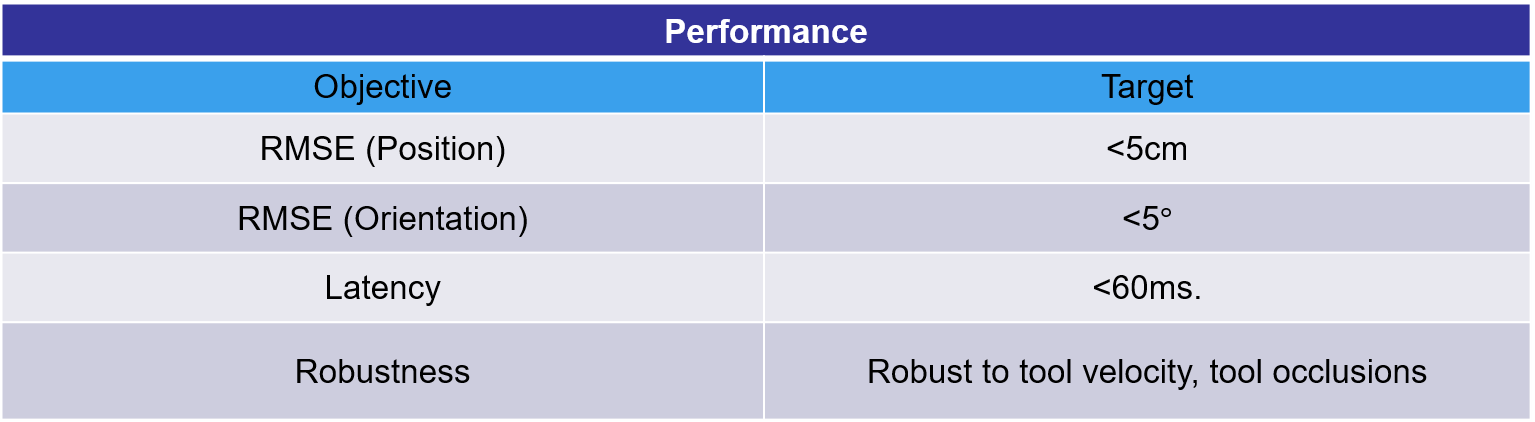
\includegraphics[width=0.8\textwidth]{Performance}
	\end{center}
	\caption{Performance design objectives}
	\label{fig:performance}
\end{figure}

The tracking system must be accurate in its position and orientation estimation to produce a high fidelity reconstruction of device movement in the user's virtual reality application. For the device to truly be a direct input device, the accuracy of the mapping between physical and virtual worlds should be as low as $1$mm, as is required for the physical and virtual registration to be imperceptible \cite{ribo2001}. In virtual reality, as opposed to augmented reality, the accuracy constraint can be relaxed somewhat. The input device will be usable as long as movements are precise and repeatable, as is the case with indirect input devices. Thus position error of about $5$\% along each axis of the trackign volume is acceptable, leading to an accuracy target of $5$cm. For orientation, device usability studies have shown that physical and virtual orientation differences of $5\degtwo$ are imperceptible to a user \cite{hinckley1997}. Therefore, the target for orientation estimation is an accuracy better than $5\degtwo$. 

\medskip

To quantify the accuracy, the root-mean-squared error model is used. The root-mean-squared error (RMSE) is the square root of the variance between the estimated values and the position or orientation reference. This error model is useful because it can be decomposed into bias and variance components.

\medskip

Requirements for low latency and high robustness fill out the design specifications. The latency should be as low as possible since the discrepency between virtual motion and physical motion has been known to induce simulator sickness in virtual environments \cite{kolasinski1995}. Best practices place the maximum latency that is comfortable for a user at 60ms \cite{oculusbest}. As far as robustness, the tracking of the device should be robust to tool occlusions and tool velocities. This will ensure that the user has control of the device in the virtual environment at all times, no matter how the tool is configured or moved in the physical environment.


%%%%%%%%%%%%%%%%%%%%%%%%%%%%%%%%%%%%%%%%%%%%%%%%%%%%%%%%%%%%%%%%%%%%%%%%%%%%%%%
%% Tracking system design
%%%%%%%%%%%%%%%%%%%%%%%%%%%%%%%%%%%%%%%%%%%%%%%%%%%%%%%%%%%%%%%%%%%%%%%%%%%%%%%

\section{Design Approach}


\subsection{Requirements}
In order to enable direct input with the interaction tool, the tool's tracking system must estimate both the position and orientation of the interaction tool. Additionally, rendering a virtual representation of the tool requires measuring its position and orientation relative to the virtual reality display orientation, given by the attitude matrix $\Ad$. To track the tool's absolute trajectory, its position is determined relative to the world -- that is, relative to a non-accelerating, inertial coordinate system in the user's physical environment. The position and orientation of the tool in the world coordinates of the inertial frame are $\pf$ and $\At$, respectively. The position of the tool in the coordinate frame of the virtual reality display is denoted by a 'prime' sign: the tip or front of the tool in display coordinates is $\pfpr$. Thus, there are four tracking targets: $\pf$, $\At$, $\pfpr$, and $\Ad$; these are shown in Figure \ref{fig:requirements}. 

\begin{figure}[H]
	\begin{center}
		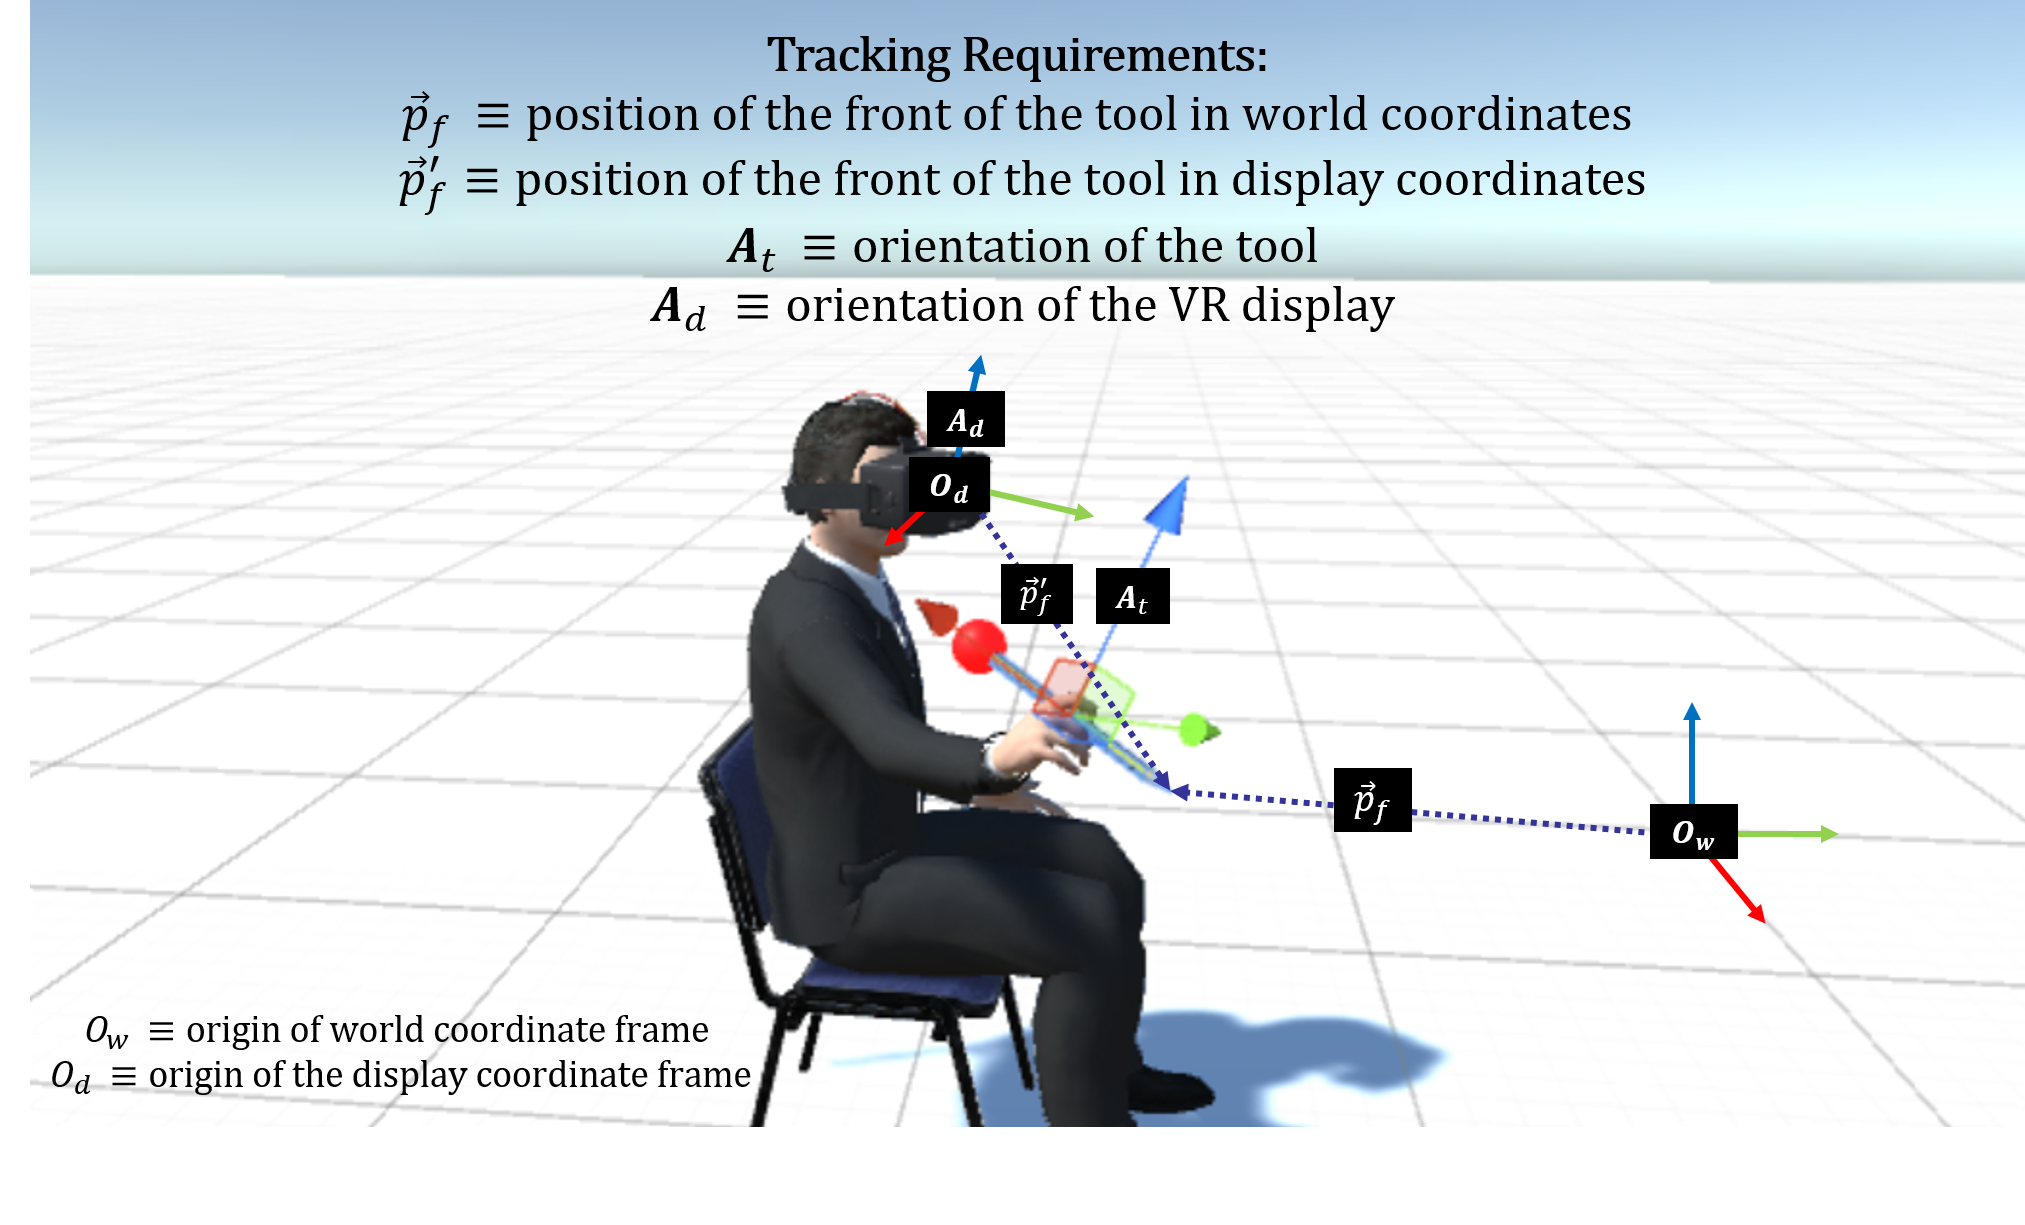
\includegraphics[width=1\textwidth]{requirements}
	\end{center}
	\caption{Position and orientation tracking requirements}
	\label{fig:requirements}
\end{figure}

\subsection{Geometry}

The geometry of the tool tracking system affects both the usability and the performance of the interaction tool. The display-referenced geometry is chosen because it eliminates the burden on the user to pre-calibrate their environment before providing direct input to VR applications. At the same time, this geometry is compatible with VR applications with which a user interacts while seated.

\subsubsection{Option 1: World-referenced geometry}

The world-referenced tracking geometry is shown in Figure \ref{fig:worldtopo}.

\begin{figure}[H]
	\begin{center}
		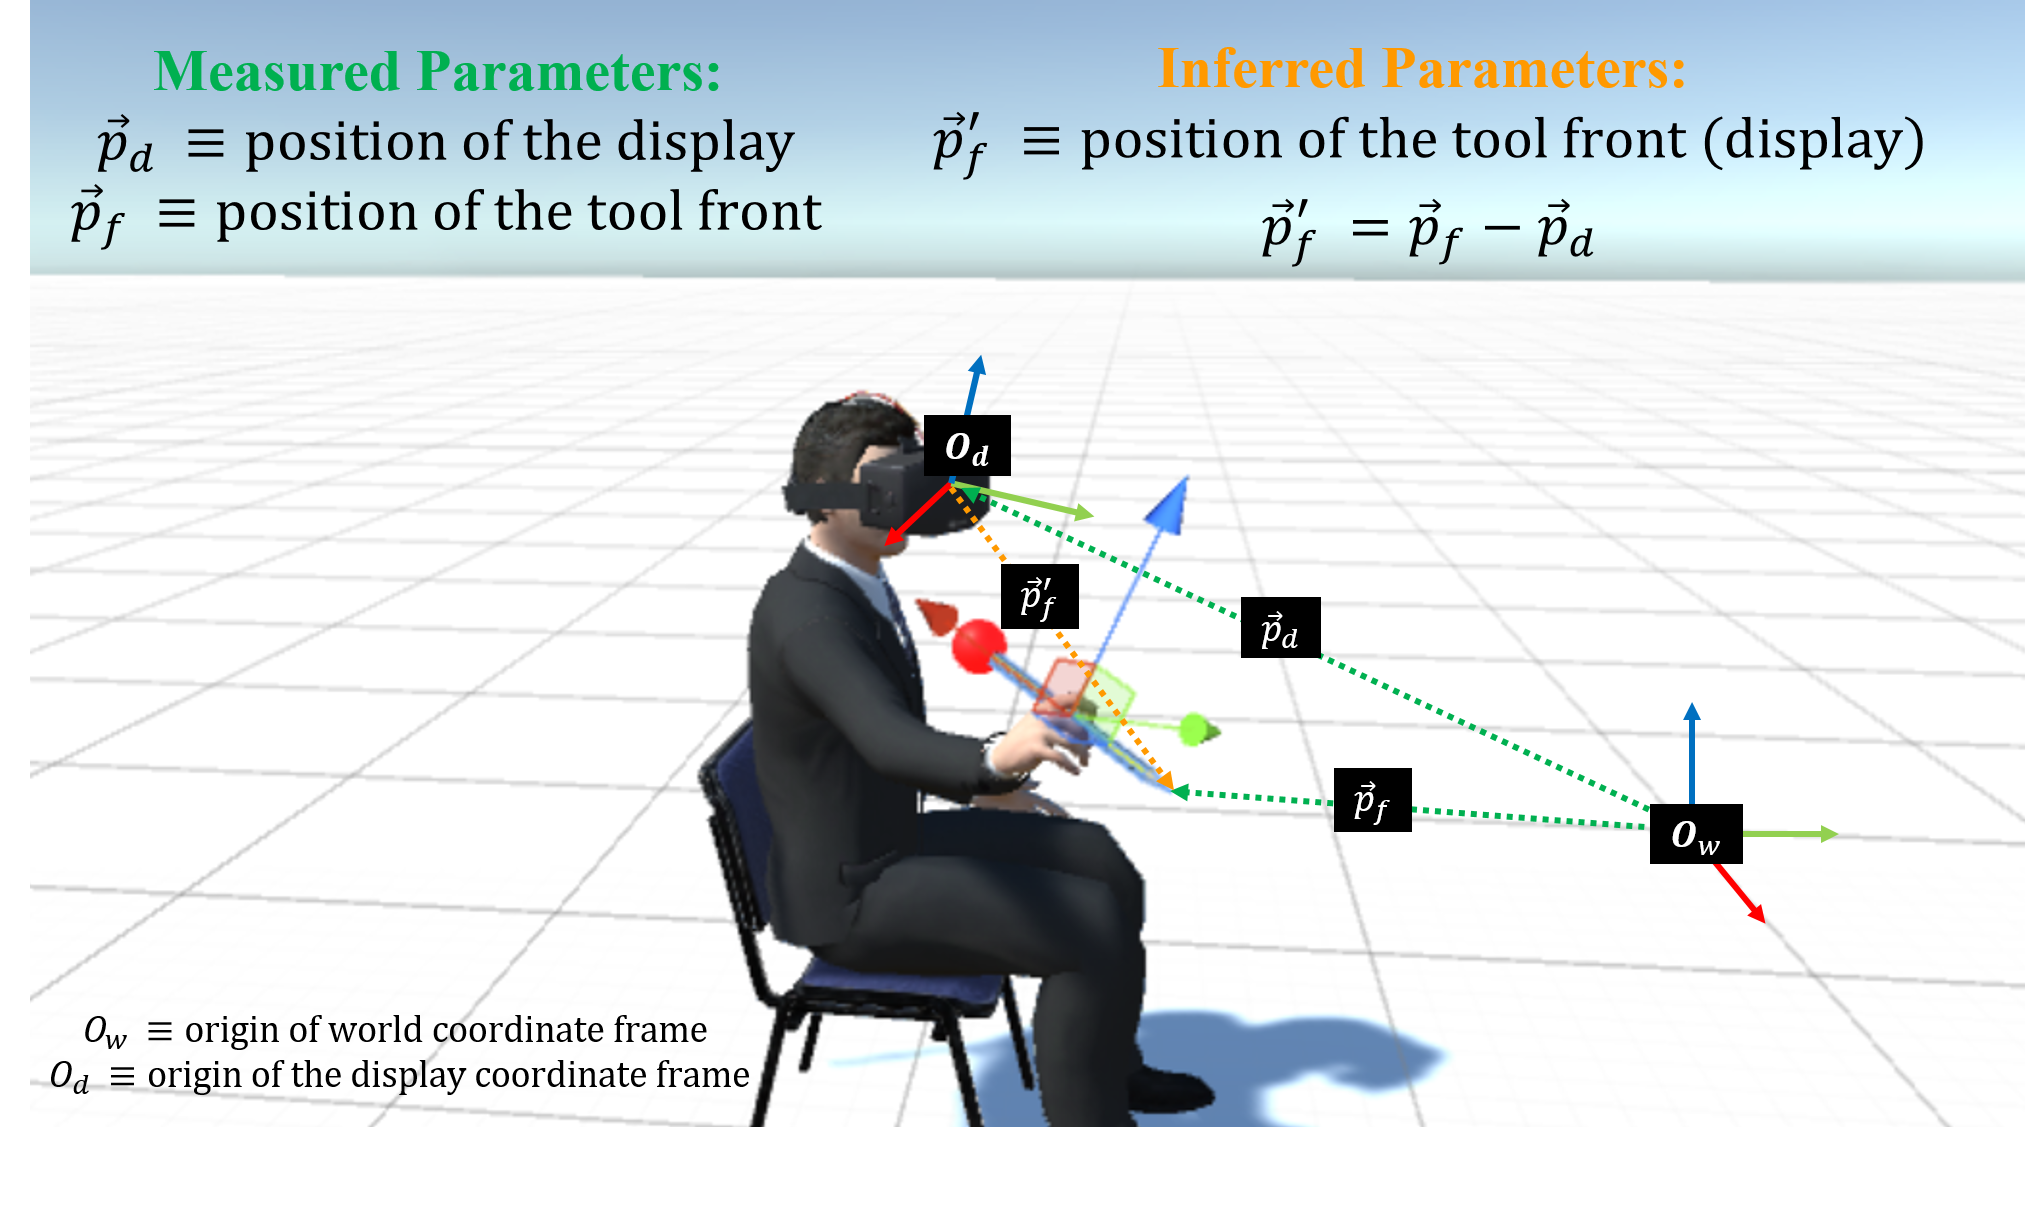
\includegraphics[width=1\textwidth]{WorldTopo}
	\end{center}
	\caption{Position tracking with a world-referenced geometry}
	\label{fig:worldtopo}
\end{figure}

\subsubsection{Option 2: Display-referenced geometry}

The display-referenced tracking geometry is shown in Figure \ref{fig:displaytopo}.

\begin{figure}[H]
	\begin{center}
		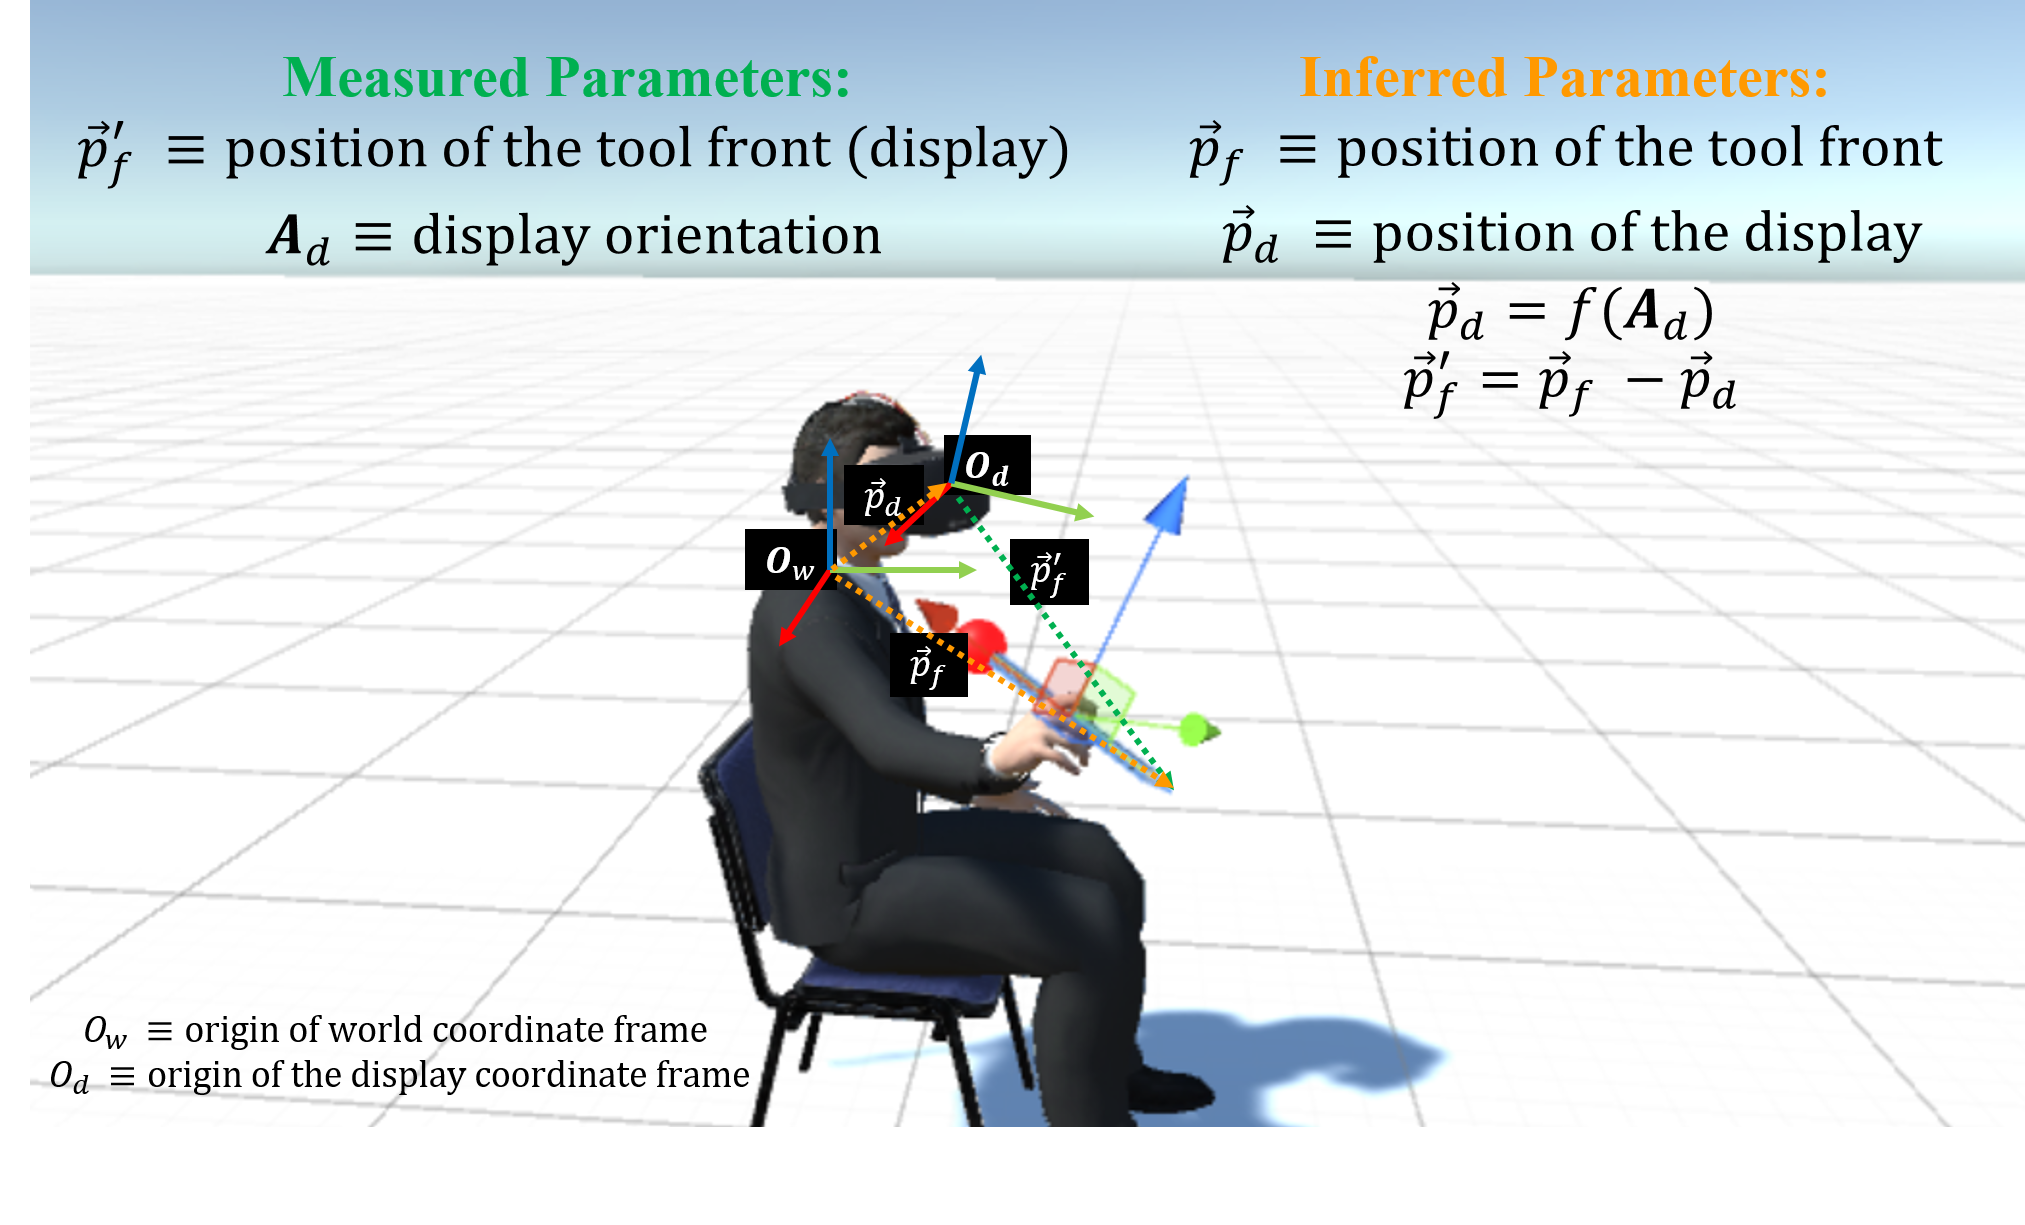
\includegraphics[width=1\textwidth]{DisplayTopo}
	\end{center}
	\caption{Position tracking with a display-referenced geometry}
	\label{fig:displaytopo}
\end{figure}

\subsubsection{Evaluating Tracking Geometries: Comparing portability and tracking volume}

Tracking geometries 1 and 2 have advantages and disadvantages when evaluated according to the usability design objectives. Relative to the usability criteria, the two geometries differ greatly in their portability and tracking volume. 

\medskip

The world-referenced tracking geometry requires a fixed coordinate system in the user's physical environment, decreasing portability by increasing the configuration overhead for using the direct input device. However, once this coordinate system is established, the user can provide direct input to a VR application over a very large tracking volume, up to the size of the room in which the tracking system is located. The display-referenced geometry, on the other hand, has the advantage of enabling a user to provide direct input to a VR application without pre-calibrating the physical environment in which they are using the VR display. The trade-off is that the tracking volume is small. Since the origin of the world coordinate system in the display-referenced geometry is located beneath the user's head, the user must remain seated while using a direct input device with a display-referenced tracking geometry.

\medskip

As discussed previously, \textit{portability} is preferred to \textit{mobility} in order to make the input device compatible with low-cost VR displays that are also highly portable.

\subsection{Technology}

A combination between optical and inertial sensors was chosen to track the 3D Interaction Tool's position and orientation. The chart in Figure \ref{fig:trackingtech} summarizes the comparison between various alternatives for the choice of the tracking technology.

\begin{figure}[H]
	\begin{center}
		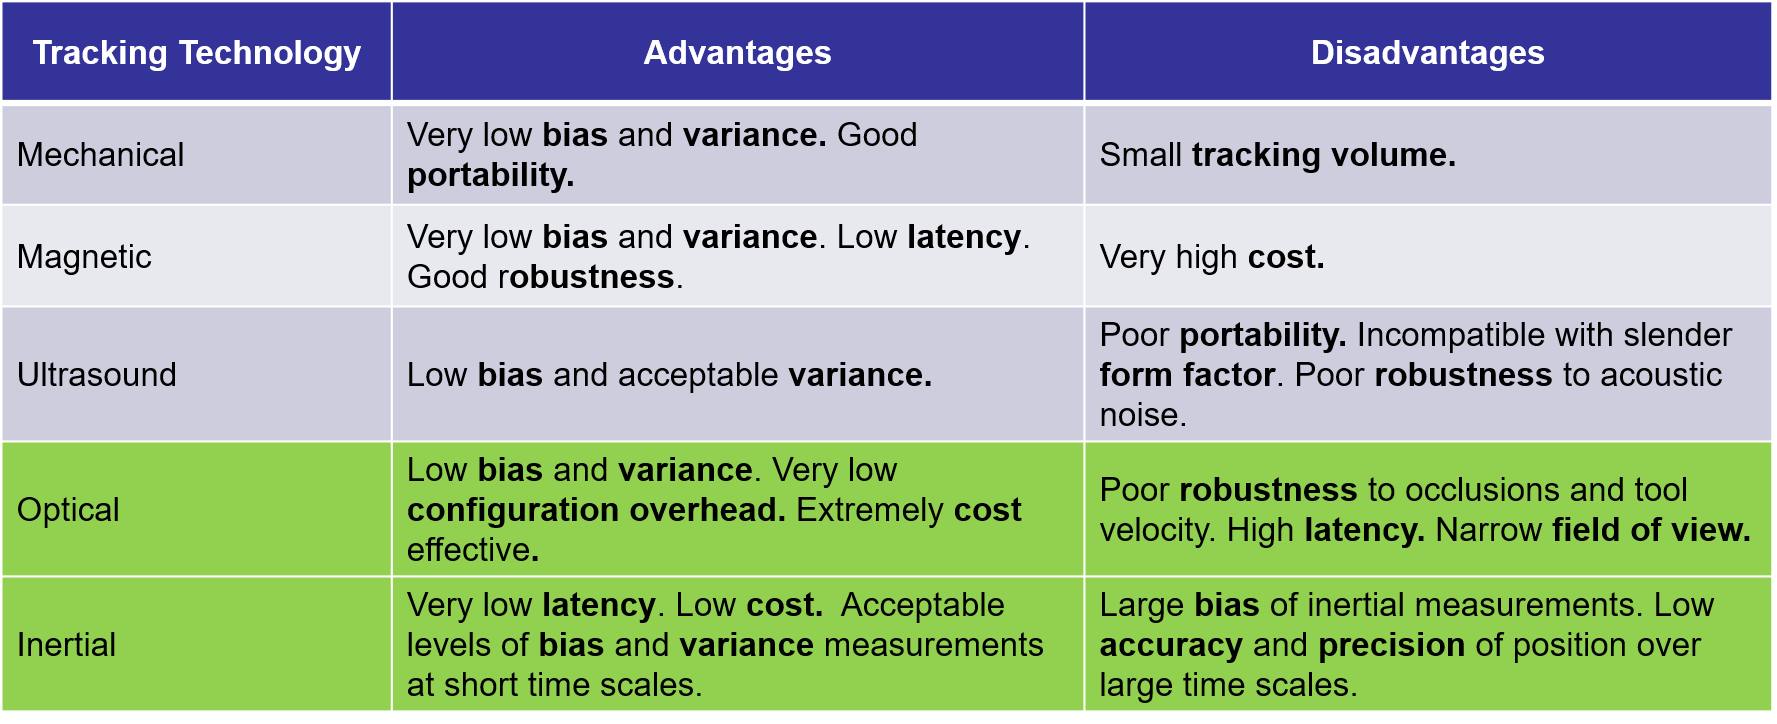
\includegraphics[width=0.8\textwidth]{TrackingTech}
	\end{center}
	\caption{Comparison of five tracking technologies}
	\label{fig:trackingtech}
\end{figure}

Magnetic and mechanical sensors were quickly eliminated as tracking options due to the high cost of the former and the limited tracking volume of the latter. Acoustic sensors were considered but rejected due to suboptimal sensor geometries \cite{rolland2001}. These geometries were incompatible with the slender design of the interaction tool.

%%%%%%%%%%%%%%%%%%%%%%%%%%%%%%%%%%%%%%%%%%%%%%%%%%%%%%%%%%%%%%%%%%%%%%%%%%%%%%%
%% Final Design
\subsection{Final Design}

\subsubsection{System Overview}

The final system layout is shown in figure \ref{fig:finaldesign}. The genius of this design is that it is completely robust to tool occlusions, provided that the user is holding the interaction tool as they would a pen or stylus. In this geometry the back of the interaction tool, which is the tracking target of the camera, is always in view. Moreover, this design achieves a large tracking volume because it only requires that the viewpoint of the user be directed in the general direction of the interaction tool for the tracking camera to find the tool in its field of view. This is possible because the display and the tracking camera are collocated. 

\begin{figure}[H]
	\begin{center}
		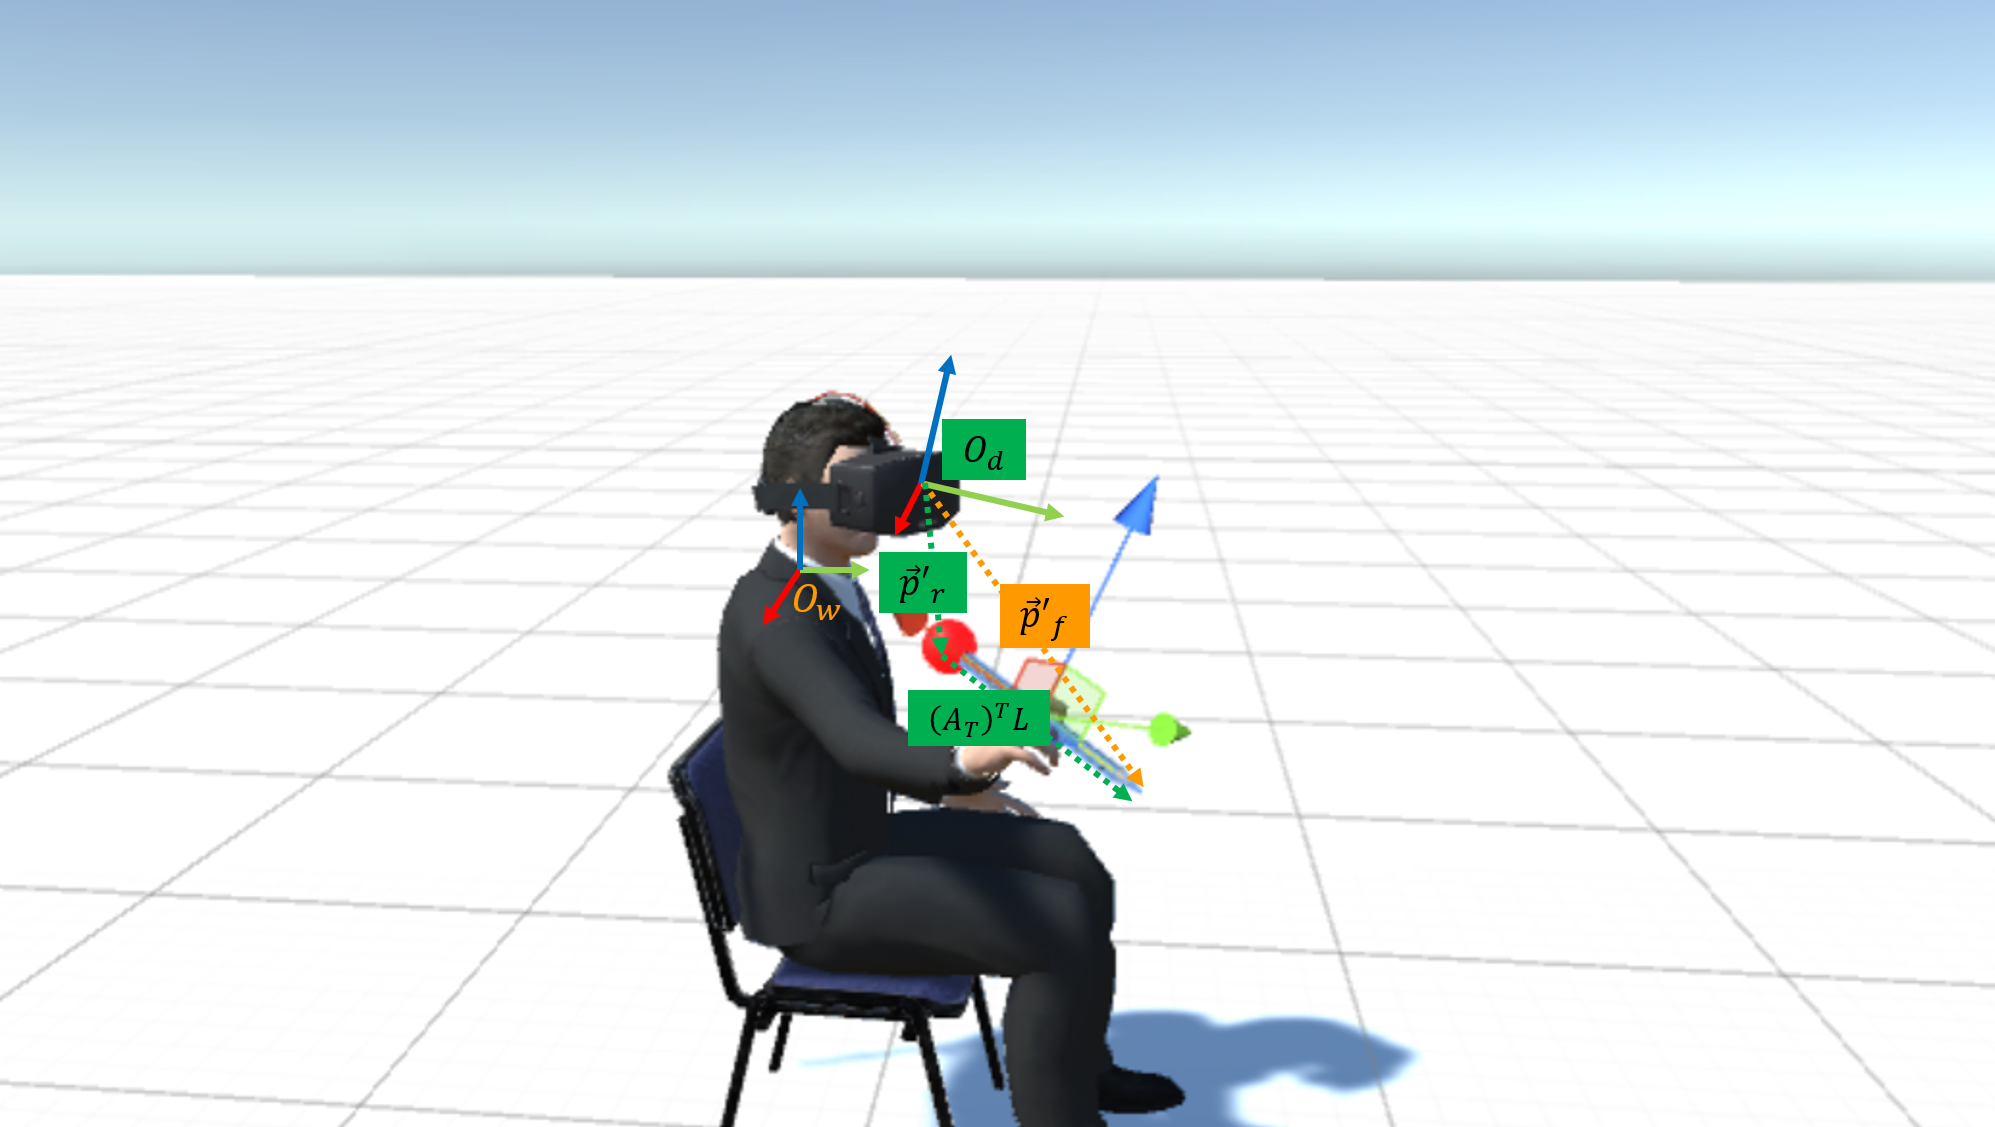
\includegraphics[width=0.8\textwidth]{FinalDesign}
	\end{center}
    \caption{Final tracking system design: a display-referenced tracking topology}
	\label{fig:finaldesign}
\end{figure}

However, one of the downsides of this tracking design is that the position of the front of the tool $\pf$, the position of interest, is largely occluded from the field of the camera and must be inferred from the measurements of the position of the rear of the tool and the orientation of the tool. Since both error in the tracking of the tool rear $\pr$ and the tracking of the orientation of the tool $\At$ (and the span vector $\pl$) will lead to error in the estimation of the position of the end of the tool, both of these measurements must be made with as little bias and variance as possible.

%% Inferring the tool position
\subsubsection{Tracking measurements}

Not all of these three tracking targets are measured directly. The tracking targets are inferred from the measurements of the position of the rear of the interaction tool relative to the camera, the attitude of the camera, and the attitude of the tool. The position of the tool relative to the camera is denoted by $\prpr$, the attitude of the camera relative to the inertial coordinate system by $\Ac$ and the attitude of the tool relative to the inertial coordinate system by $\At$. The vector $\pspr$ is measured by finding the .

%% Inferring the tool position
\subsubsection{Inferring the tool position}

The position of the front of the tool in world coordinates is given by $\pf$. This position is inferred through measurements of the position of the rear of the tool and the tool's orientation. The equation for the position of the front of the tool is 

$$ \pf = \pr + \pl = \pr + \Atinv \plpr $$

where the position of the rear of the tool, $\pr$ is given by

$$ \pr = \Acinv \prpr - \pc $$

and $\pl$ is the span vector that relates the rear of the tool to the front of the tool -- it is essentially the length of the tool rotated from the body coordinate system of the tool to world coordinates. The attitude matrix given by, $\Atinv$, is the rotation from the body coordinates of the tool to the world coordinate system.

In order to render the tool on the display for the user, the position of the tool must be known to the VR application in the coordinate system of the VR display. The position of the front of the tool in display coordinates is $\pfpr$ and it is found by multiplying the tool's position in the world coordinate system by the attitude of the display. Additionally, the position of the display must be added to the tool position before multiplying by the display attitude matrix:

$$ \pfpr = \Ad (\pf + \pd) $$

The tool attitude in the coordinate system of the display is denoted by $\Atpr$ and it is found by composing the rotation from the tool's body coordinates to world coordinates with the display attitude matrix: 

$$ \Atpr = \Ad \Atinv \pl $$

This is the tool orientation visible to the user. 

%%%%%%%%%%%%%%%%%%%%%%%%%%%%%%%%%%%%%%%%%%%%%%%%%%%%%%%%%%%%%%%%%%%%%%%%%%%%%%%
%% Implementation
%%%%%%%%%%%%%%%%%%%%%%%%%%%%%%%%%%%%%%%%%%%%%%%%%%%%%%%%%%%%%%%%%%%%%%%%%%%%%%%
\section{Implementation}

The system's physical layout is shown in \ref{fig:systemlayout}. For simplicity, the tracking camera is assumed to be fixed. The model for this system is geometrically equivalent to the one presented in Figure \ref{fig:finaldesign}. The webcam of the computer is used as the tracking camera. The inertial measurement unit, the Adafruit BNO055, is attached to the breadboard. The Adafruit sensor was chosen because it has built-in calibration routines for its three sensors: an accelerometer, a gyroscope, and a magnetometer. Since all of these sensors have bias that must be subtracted off, the calibration routines of the BNO055 are of great help to the prototyping process. 

\medskip 

A colored foam sphere is attached to the rear of the interaction tool to serve as the tracking target for the camera.

\begin{figure}[H]
	\begin{center}
		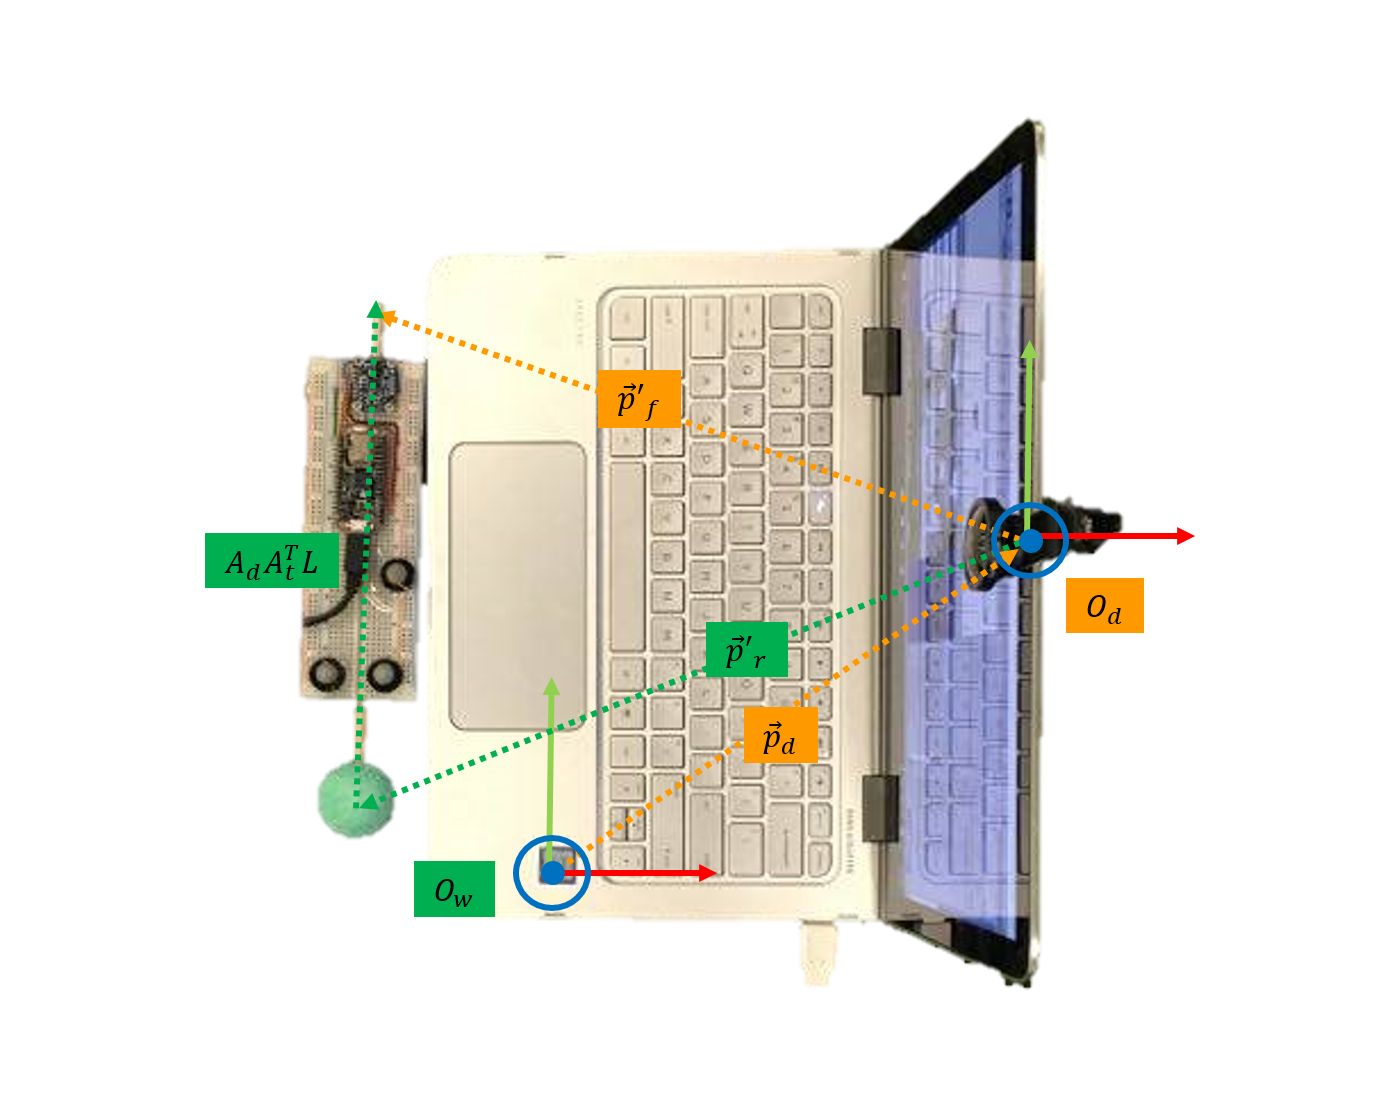
\includegraphics[width=0.8\textwidth]{SystemLayout}
	\end{center}
    \caption{Geometrically equivalent tracking system}
	\label{fig:systemlayout}
\end{figure}

The virtual reality application runs on the computer shown in Figure \ref{fig:systemlayout}. While this virtual reality application is not immersive, it creates a virtual 3D environment displayed to the user on the computer screen, where they can interact with virtual objects. Thus, this geometry is sufficient to prove the usefulness of the 3D Interaction Tool for virtual reality applications.

\medskip

The spherical tracking target is chosen because its size in each image does not depend on its orientation. Additionally, if the angle subtended by the tracking target in the field of view is small, then the midpoint of the tracking target in world coordinates is on the same plane as the vanishing points on the edges of the target.

\medskip

The block diagram of the implemented tracking system is shown in Figure \ref{fig:systemdiagram}.

\begin{figure}[H]
	\begin{center}
		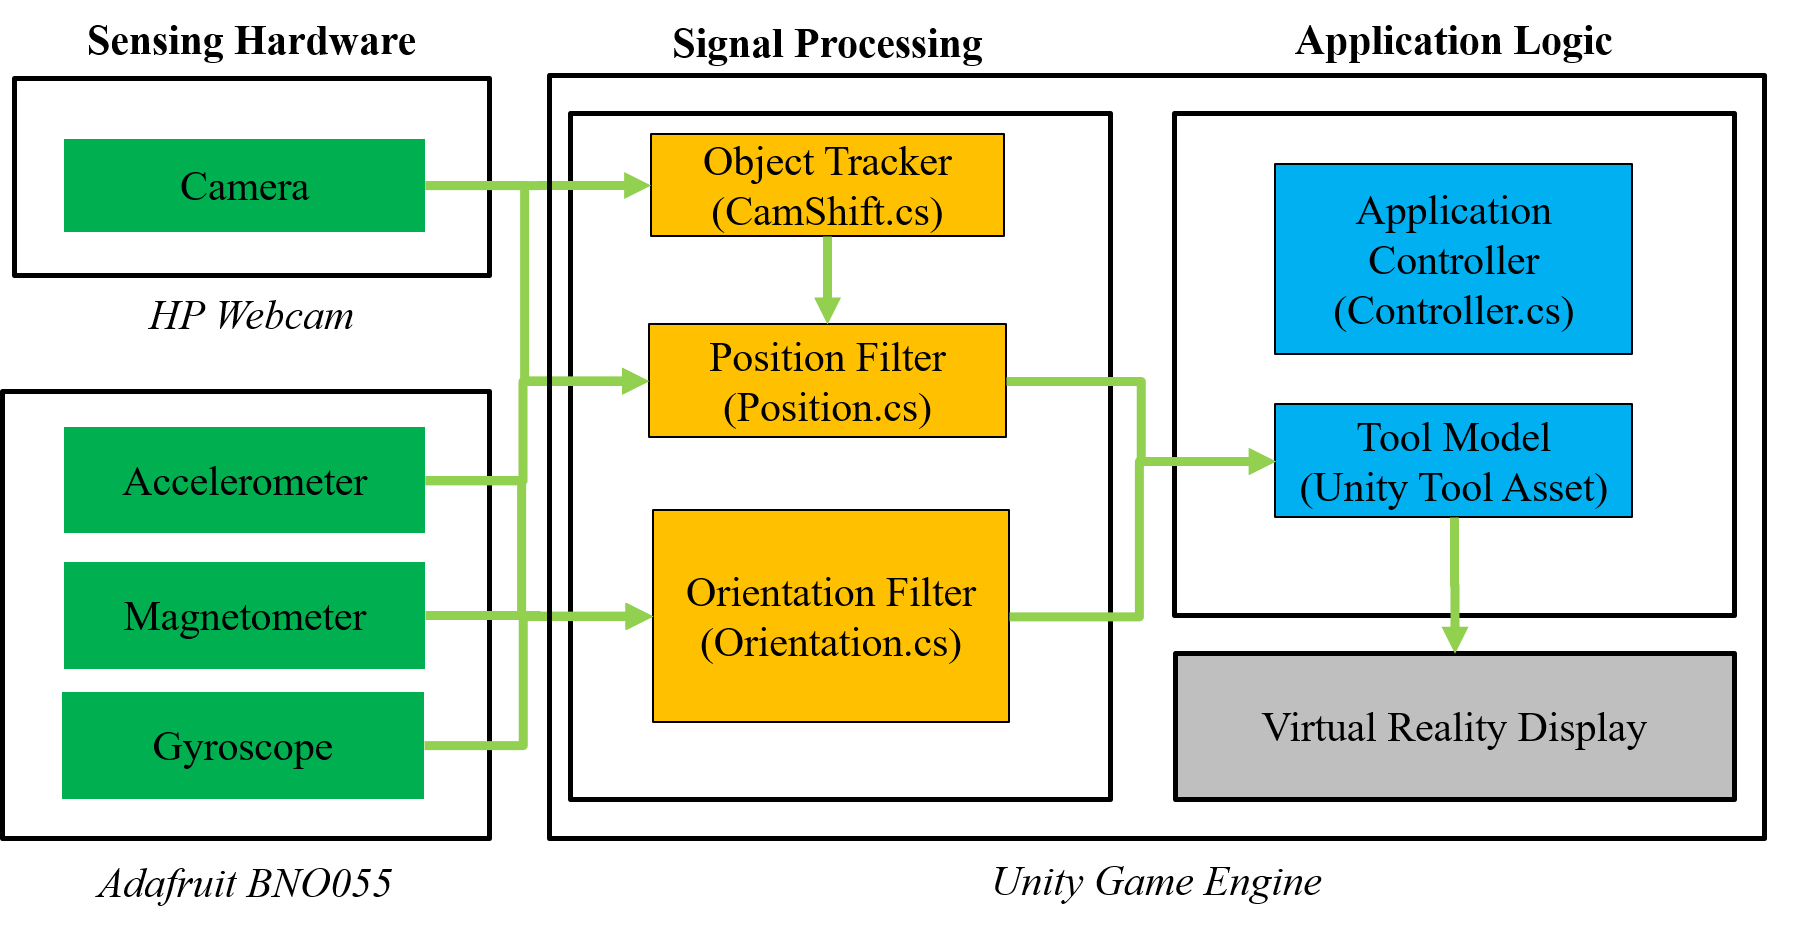
\includegraphics[width=0.8\textwidth]{SystemDiagram}
	\end{center}
    \caption{Full system diagram of implementation}
	\label{fig:systemdiagram}
\end{figure}

The files referenced with the extension 'cs' are included with the code repository of this report at \url{https://github.com/lgemar/thesis}. 

%%%%%%%%%%%%%%%%%%%%%%%%%%%%%%%%%%%%%%%%%%%%%%%%%%%%%%%%%%%%%%%%%%%%%%%%%%%%%%%
%% Orientation tracking
%%%%%%%%%%%%%%%%%%%%%%%%%%%%%%%%%%%%%%%%%%%%%%%%%%%%%%%%%%%%%%%%%%%%%%%%%%%%%%%
\section{Orientation Tracking}

The orientation of the interaction tool must be estimated to find the span vector, $\pl = \pf - \pr = \At \plpr$. The naive approach for estimating the orientation of the tool is to start with two known vectors in the reference coordinate system -- the gravity vector and the earth's magnetic field vector are good candidates. Then we can find the attitude matrix directly by sensing these two reference vectors in the body coordinates of the device and finding the rotation matrix that maps them back to the reference coordinate frame. While this method is computationally and conceptually simple, the estimation is very sensitive to noise from both the accelerometer and the magnetometer that sense the gravity and magnetic field vectors, respectively. We would like some way of filtering these estimates in real-time. Before investigating a real-time orientation tracking filter, the results of the TRIAD measurement model are presented for comparison.

\subsection{Naive Measurement Model: TRIAD}

The TRIAD estimation method finds the attitude matrix $A$ that maps three reference frame vectors $\vec{r}_k$ to their corresponding body frame vectors $\vec{b}_k$ for $k = 1, 2, 3$ \cite{Shuster2004}. Two observations of reference frame vectors provide sufficient information to compute a right-handed orthonormal triad of vectors in the reference frame. If $\vec{v}_1$ and $\vec{v}_2$ are reference frame vectors for the accelerometer and the magnetometer, respectively so that the gravity vector points down and the magnetometer vector points in the direction of magnetic North in Boston, relative to the world reference frame. The orthonormal vector triad representing the reference frame is given by, 

$$ 	\vec{r}_1 = \frac{\vec{v}_1}{\| \vec{v}_1 \|}, \tab \vec{r}_2 = \frac{\vec{v}_1 \times \vec{v}_2}{\| \vec{v}_1 \times \vec{v}_2 \|}, \tab \vec{r}_3 = \vec{r}_1 \times \vec{r}_2 $$

Let $\vec{w}_1$ be the measurement of the normalized unit vector from the accelerometer and $\vec{w}_2$ be the measurement of the normalized unit vector from the magnetometer, then the orthonormal vector triads for the reference vectors are given by, 

$$ \vec{b}_1 = \frac{\vec{w}_1}{\| \vec{w}_1 \|}, \tab \vec{b}_2 = \frac{\vec{w}_1 \times \vec{w}_2}{\| \vec{w}_1 \times \vec{w}_2 \|}, \tab \vec{b}_3 = \vec{w}_1 \times \vec{w}_2 $$

If there was no noise in the system, then it would be the case that $\vec{b}_k = A \vec{r}_k$ for $k=1,2,3$. An equivalent way of writing this in matrix form is the following: 

$$ M_b = A M_r $$ 

where 

$$ M_b = \mat{ \vec{b}_1 & \vec{b}_2 & \vec{b}_3 } $$
$$ M_r = \mat{ \vec{r}_1 & \vec{r}_2 & \vec{r}_3 } $$

Since $M_r$ is an orthogonal matrix, its inverse is equal to its transpose: $M_r^{-1} = M_r^{T}$. Thus, the solution for the attitude matrix is, 

$$ A = M_b M_r^{T} $$

\subsubsection{Error Analysis of TRIAD Measurements}

There are three independent maneuvers that are possible with the interaction tool: roll maneuvers, pitch maneuvers, and yaw maneuevers. The error analysis focuses on the pitch maneuver but similar results are obtained for a rotation of the interaction tool in any dimension. Using the TRIAD algorithm, the roll, pitch, and yaw angles are estimated, and these are seen side-by-side with the absolute orientation reference in Figure \ref{fig:pitchmaneuver}. 

\begin{figure}[H]
	\begin{center}
		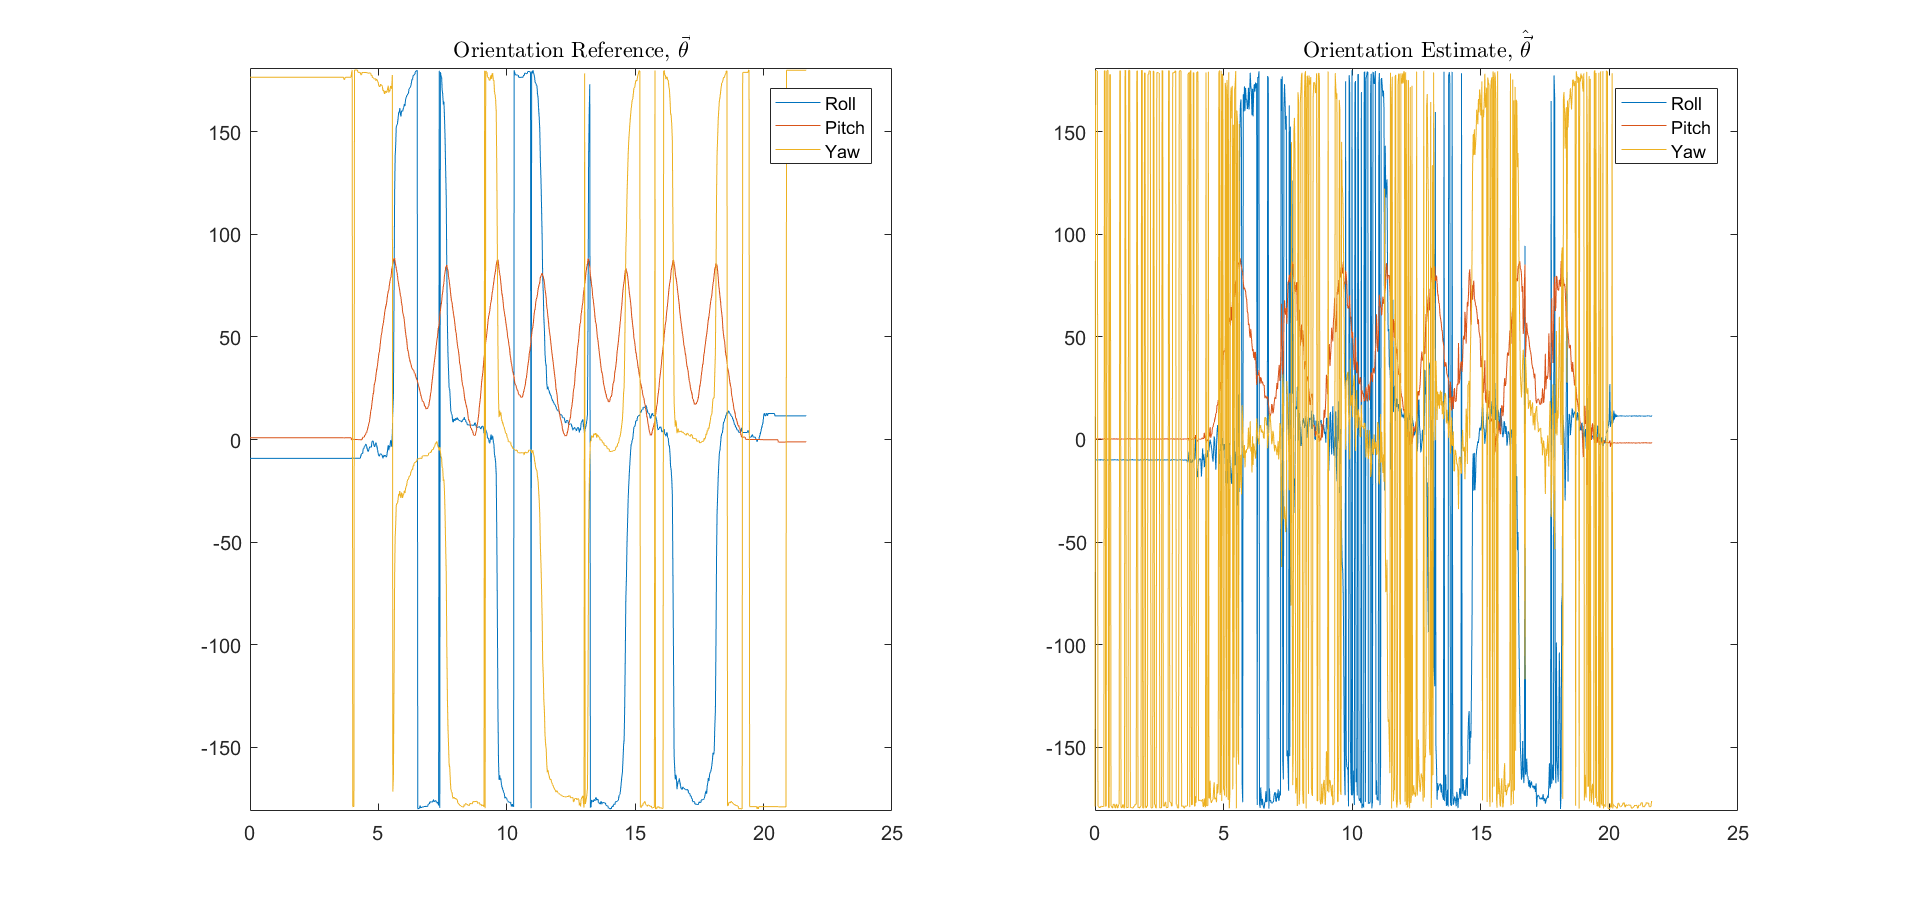
\includegraphics[width=1\textwidth]{PitchManeuver}
	\end{center}
    \caption{Pitch maneuver reference versus estimates}
	\label{fig:pitchmaneuver}
\end{figure}

The error associated with the estimation of roll, pitch, and yaw is shown in \ref{fig:pitcherrortriad}.

\begin{figure}[H]
	\begin{center}
		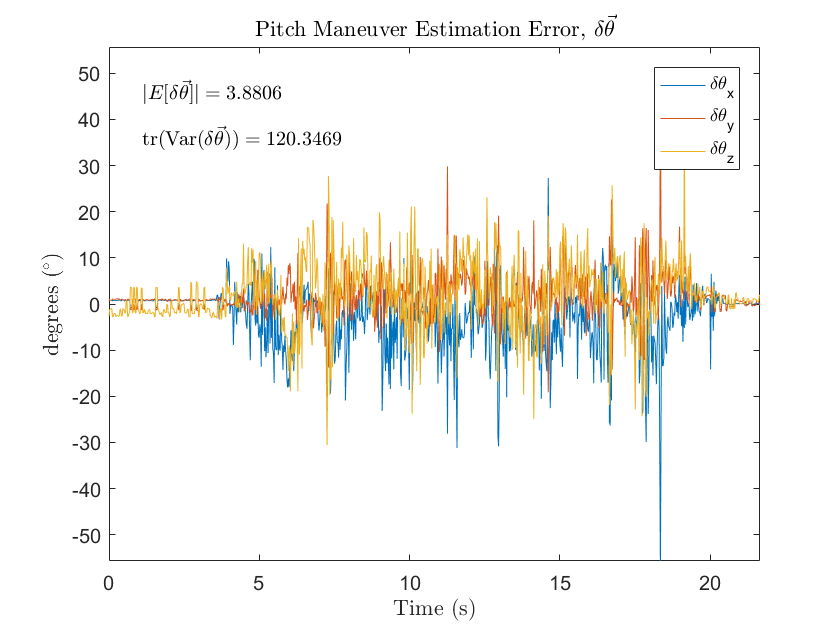
\includegraphics[width=1\textwidth]{PitchManeuverTriad}
	\end{center}
    \caption{Pitch error for TRIAD estimation}
	\label{fig:pitcherrortriad}
\end{figure}

The bias of the measurements is just $4.3 \degtwo$ but the variance is more than $125 \degtwo$, corresponding to a root-mean-squared error of $11.2\degtwo$. If a user notices an angular change of $5\degtwo$, a deviation of more than $10\degtwo$ is likely to give them a headache. Similar results are obtained when analyzing maneuvers in the roll and yaw dimensions of the rotation. These errors and root-mean-squared errors are summarized in the table of Figure \ref{fig:triaderrorsummary}.

\begin{figure}[H]
    \begin{center}$
        \begin{array}{cc}
            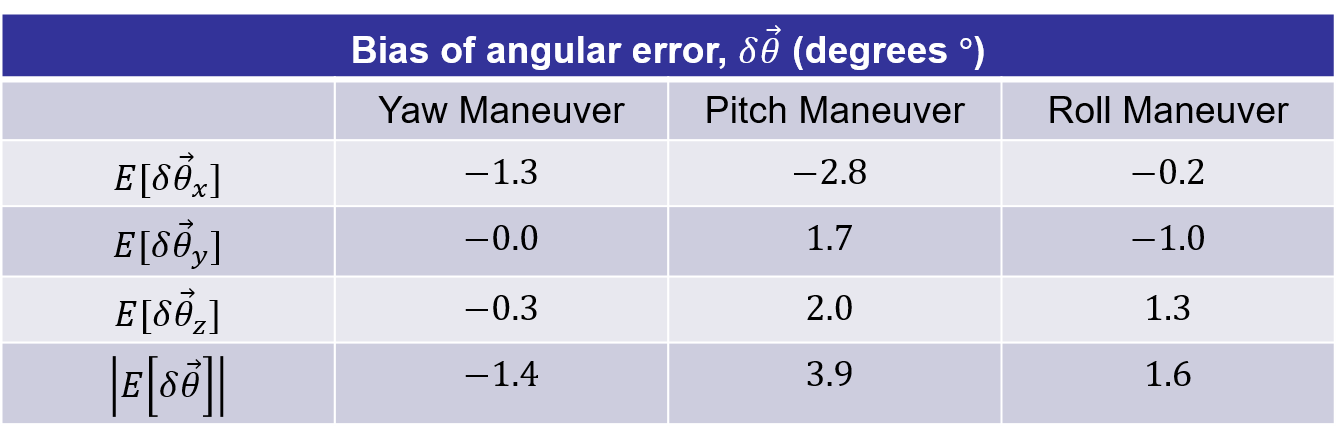
\includegraphics[width=0.7\textwidth]{TriadBias} \\
            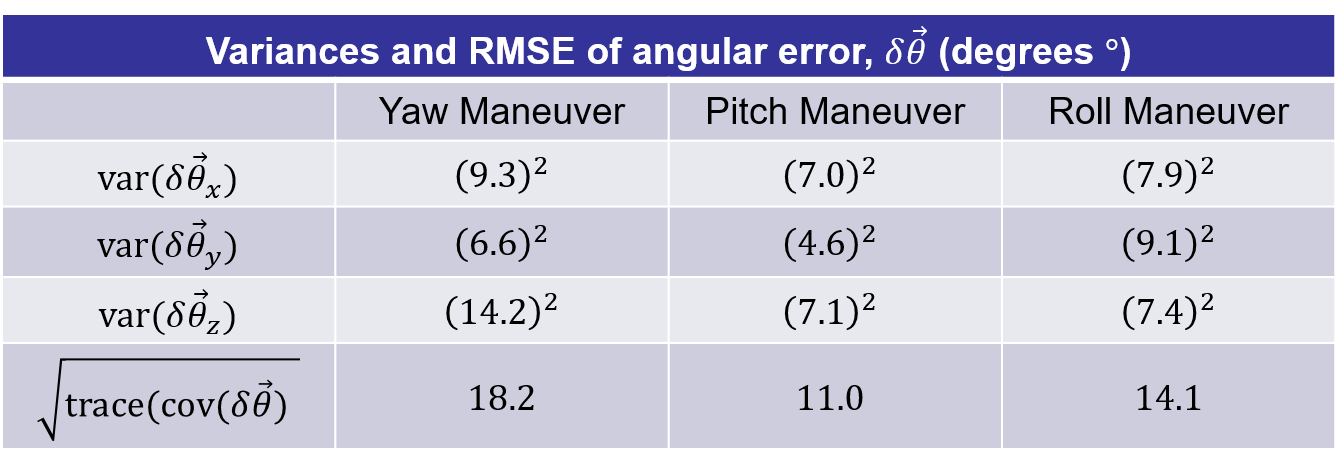
\includegraphics[width=0.7\textwidth]{TriadVariance}
        \end{array}$
    \end{center}
    \caption{TRIAD orientation tracking errors}
    \label{fig:triaderrorsummary}
\end{figure}

Notice that the yaw maneuver suffers from the greatest root-mean-squared error (RMSE). The yaw maneuver is particularly difficult to track due to the unreliability of the magnetometer sensor and this will be a theme throughout the remainder of the error analysis. 

\subsection{Improving the Orientation Estimation}

The error of the TRIAD estimation routine is 2-3x times the targets presented in \ref{fig:performance}. Therefore, we would like to find a way to decrease the variance of the orientation estimation without increasing the latency of the system. To do this we need a real-time estimator. Any optimal real-time estimator for this system should incorporate all the information we know about the system. Note that the TRIAD method used only the accelerometer and magnetometer information from the inertial sensor and neglected the data from the gyroscope. 

Is there a way that we can use the data from the gyroscope to improve the orientation estimation? In fact there is! But it requires that we related the gyroscope measurements to the dynamics of rotation. This is not a simple problem for three reasons. First, rotations are non-linear and therefore the dynamics are non-linear. Second, any 3-dimensional parameterization of the rotations for purposes of writing down a non-linear model contains a singularity and we must use a higher dimensional parameterization of the rotation \cite{stuelpnagel1964}.

Singularities in the three-dimensional representation of rotations are not problematic for small rotations. However, they are problematic for the 3D Interaction Tool because the user of the interaction tool is free to move the device into any orientation. This means that the tool can be held in any orientation, and the changes in the orientation are potentially extremely large. 

\subsection{Mathematical Representation of Orientation}

The orientation of the interaction tool relative to the world coordinate frame can be represented in a number of ways. The two representations that will be important here are the attitude matrix and the attitude quaternion. First, the attitude of the orientation tool can be described by the attitude matrix $A$. The attitude matrix typically maps a vector in the reference frame to a vector in the the body frame \cite{Markley2007}. This mapping is given by the relation, 

\[ \bf{b} = A \bf{r} \]

Second, the attitude of the interaction tool can be represented as a quaternion. A rotation in three-dimensions is equivalent to an axis of rotation and and angle of rotation. If $\hat{n}$ is the axis of a rotation and $\theta$ is the angle of the rotation, then the quaternion $\overline{q}$ represents the attitude: 

\[ \overline{q} = \mat{\vec{q} \\ q_4} \] 

with $\vec{q} = \hat{n} \sin{\frac{\theta}{2}}$ and $q_4 = \cos{\frac{\theta}{2}}$. The quaternion must have length 1: $\overline{q}^T \overline{q} = 1$. 

The attitude matrix and the quaternion representing attitude are related by the following equation, where $A$ is a function of $\overline{q}$ \cite{Shuster1982}: 

\[ A(\overline{q}) = (q_4^2 - {\| \vec{q} \|}^2) I_{3x3} + 2 \vec{q}\vec{q}^T - 2 q_4 [\vec{q}\times] \]

where ${[\vec{q}\times}]$ is the skew-symmetric cross product matrix, 

\[ [\vec{q}\times] = \mat{ 0 & -q_3 & q_2 \\ q_3 & 0 & -q_1 \\ -q_2 & q_1 & 0} \]

The relationship between $A$ and $\overline{q}$ can also be expressed as the product of two matrices \cite{Markley2007}: 

\[ A(\overline{q}) = \Xi(\overline{q})^{T} \Psi(\overline{q}) \]

with 

\[ \Xi(\overline{q}) = \mat{q_4 \bf{I}_{3x3} + [\vec{q}\times] \\ -\vec{q}^T } \]

\[ \Psi(\overline{q}) = \mat{q_4 \bf{I}_{3x3} - [\vec{q}\times] \\ -\vec{q}^T } \]


\subsection{Dynamic Measurement Model}

The rate of change of the attitude can be written in the form of a general state space model: 

\[ \dot{\vec{x}} = A(\vec{x}, t) \vec{x} + B(\vec{x}, t) \vec{u} \]

The kinematic equation for the change in attitude as a function of the angular rate can be written as a rate of change of the attitude matrix or a rate of change in the quaternion \cite{Shuster1982}. The angular velocity vector is given by $\vec{\omega}$. The rate of change of the attitude matrix is, 

\[ \dot{A}(t) = [\vec{\omega}\times] A(t) \]

In this equation, $[\vec{\omega}\times]$ is an instance of the state transition matrix $A(\vec{x}, t)$ from the general schema for a state space model. The kinematic relation for the rate of change of the quaternion can be written in the following two ways: 

\[ \dot{\overline{q}} = \frac{1}{2} \Omega( \vec{\omega} ) \overline{q} \]

\[ \dot{\overline{q}} = \frac{1}{2} \Xi( \overline{q} )\vec{\omega} \]

where the first relation is a state space model with state transition matrix $A(\vec{\omega}) = \Omega(\omega)$, where the state transition matrix is a function of the angular rate vector $\vec{\omega}$:

\[ \Omega(\vec{\omega}) = \mat{ -[\vec{\omega}\times] & \vec{w} \\ -\vec{\omega}^T & 0 } \] 

The second kinematic equation for the rate of change of the quaternion is an instance of the schema for the state space model where the angular rate $\vec{\omega}$ is treated as the input $\vec{u}$ to the system and the input matrix $B(\overline{q}) = \Xi(\overline{q})$ is a function of the current attitude $\overline{q}$. 

\medskip

There are two good reasons to use the quaternion representation of attitude: first, the rate of change of the quaternion is linearly related to the state of the quaternion; and second, successive rotations are computed by taking the product of quaternions \cite{Markley2007}. The following identity holds of the composition of quaternions \cite{Shuster1982}: 

\[ A(\overline{q}_1) A(\overline{q}_2) = A(\overline{q}_1 \otimes \overline{q}_2) \]

with the operation $A(\overline{q})$ finding the attitude matrix $A$ that corresponds with the quaternion $\overline{q}$. Following the notation in \cite{Markley2007}, the product of the quaternion is linear in each of the quaternions $\overline{q}_1$ and $\overline{q}_2$: 

\[ \overline{q}_1 \otimes \overline{q}_2 = \mat{ \Psi({\overline{q}_1}) & \overline{q}_1} \overline{q}_2 = \mat{ \Xi({\overline{q}_1}) & \overline{q}_1 } \overline{q}_2 \]

The inverse of the quaternion is found by negating the imaginary component of the quaternion: 

\[ \overline{q}^{-1} = \mat{ -\vec{q} \\ q_4 } \]

\subsubsection{Filter Design}

How does the orientation of the interaction tool change from one time step to another? To discretize the dynamic model of rotations, we must know how the orientation of the tool will change between time steps. The change in orientation of the hand-held tool over time must be dependent on the dynamics of wrist movement. The peak velocity for human wrist movements is on the order of $10^2 \frac{\degtwo}{s}$ for fast and accurate wrist rotations \cite{hoffman1986}. We can assume that users of the interaction tool will pursue accurate movements from one orientation to another and not move the tool wildly. Therefore, the change in the orientation of the tool betweeen time steps for maximum angular velocity movements will be on the order of $2 \degtwo$, given a sample rate of $50$ Hz. This rotation is so small as to be imperceptible to most users \cite{hinckley1997}. Given these assumptions, we can assume that the orientation of the tool is more or less fixed between samples and we can treat changes to the orientation as solely due to small deviations -- essentially noise. 

\medskip

The small deviations in the angular velociy between samples can be approximated by integrating the angular velocity over the time step. The integrated angular velocity can be treated as a small deviation to the quaternion at time step $k$:  

$$ \dq = \mat{\frac{1}{2} \gyro \Delta t \\ 1} $$  

Thus, given this small deviation we can predict the orientation at time step $k$ given the orientation at step $k-1$: 

$$ \qkp = \dq \otimes \q_{k-1} = \mat{\Xi(\q_{k-1}) & \q_{k-1}} \dq = \q_{k-1} + \Xi(\qk) (\frac{1}{2} \gyro \Delta t) $$

Now this is our discrete-time dynamic model! The state transition matrix $F = I_{3x3}$ and the input matrix $G$ is parameterized by $\qk$ so that $G = \Xi(\qk)$. 

\medskip

In order to be able to integrate this orientation prediction with our measurements, we must also approximate the evolution of the covariance between time steps. Here the assumption that the orientation is fixed comes in handy for the covariance of the estimation does not change if the body is in a fixed configuration. However, the input from the gyroscope adds uncertainty. Let $Q$ be the process noise in the gyroscope input, then the predicted covariance at time $k$ given the covariance at step $k-1$ is 

$$ \Ppp = \mathbf{P}_{k-1} + Q $$

How do these predicted quantities relate to our measurements? Ultimately we want to be able to compute the innovation, the difference between the predicted measurements and the actual measurements. Once we multiply the innovation by the Kalman gain, we will know how to filter our prediction to produce a better estimate of the orientation. So how do we predict what will be measured? 

\medskip 

We expect that the measured gravity vector and magnetic field vector will simply be the gravity reference vector rotated into the current body coordinates of the interaction tool. Similarly, the expected measurement for the magnetic field vector depends on the tool's current orientation. Thus, we estimate that what we will measure is 

$$ \hat{z}_k = \mat{A(\qk)\vec{g} \\ A(\qk) \vec{b}} $$

Now we can compute the innovation $\mu$ as the difference between what we predicted we would measure and what we actually measure: 

$$ \mu = z_k - \hat{z}_k $$

Multiplying the innovation by the gain of the filter, $K$, we compute the update residual

$$ \dq^{+} = K \mu $$

This update residual is given as an error in the rotation of the interaction tool. Therefore instead of adding it to the predicted quaternion directly, we compose the two, as we do for rotations 

$$ \qk^{+} = \dq^{+} \otimes \qkp $$

This is the estimated orientation for time step $k$. 

\medskip

There is some subtlety to finding the filter gain $K$. The Kalman filter equations for the extended Kalman Filter give $K$ as 

$$ K = P^{-} H_k (H_k P^{-} H_k^{T} + R)^{-1} $$

but this requires that we know both the measurement noise, $R$, and the measurement sensitivity matrix $H_k$. While the measurement noise is initialized with reasonable values based on the expected noise of the sensors, the measurement sensitivity matrix changes on each time step because the errors in the measurements depend on the current orientation. It turns out that if $\hat{z}_k = h(\qk)$ then the measurement sensitivity is 

$$ H_k = \frac{\partial h}{\partial \dq} = \mat{2 A(\qk) \vec{g}^{\times} \\ 2 A(\qk) \vec{b}^{\times} } $$ 

where $\vec{g}^{\times}$ is the cross product matrix. This measurement sensitivity matrix is the linearization of the rotation around the current orientation. This result will be derived in the later section on the overall performance analysis of the tracking system.


% Extended Kalman Filter Initialization
\subsubsection{Filter Initialization}

The initial state of the orientation is estimated using the TRIAD approach. The rotation matrix output of the TRIAD approach is converted to a quaternion to initialize the dynamic model. In order to inialize the covaraince, an initial uncertainty in the orientation of 10 degrees is assumed. 

\medskip

The Kalman filter assumes process noise and measurement noise in the dynamics. The process noise for the dynamic model of rotations assumes that the body is fixed at each time step, so the noise in the dynamics must come from noise on the gyroscope input. The root-mean squared noise density of gyroscope on the the Adafruit BNO055 given in the data sheet as $0.014 \frac{\frac{\degtwo}{s}}{\sqrt{\Hz}}$ \cite{bnO055datasheet}. To find the mean squared noise, this value is squared and multiplied by bandwidth of the signal, taken here to be the sample rate, $47$ Hz. This yields a value of approximately $(0.1)^2 \frac{\degtwo}{s}$. Converting to radians, the mean squared noise of the gyroscope is $2.8\mathrm{e}{e-6} \frac{rad}{s}^2$. Thus, the process noise $Q$ is initialized as 

$$ Q = \mat{2.8\mathrm{e}{e-6} & 0 & 0 \\ 0 & 2.8\mathrm{e}{e-6} & 0 \\ 0 & 0 & 2.8\mathrm{e}{e-6}} $$

\medskip

Similarly, the measurement noise is initialized with noise values for the accelerometer and magnetometer listed in the datasheet \cite{bnO055datasheet}. Again, squarinng the noise densities and multiplying by the bandwidths yields mean squared errors of $1.1\mathrm{e}{e-6} g^2$ and $17 \mu T^2 $ for the accelerometer and the magnetometer, respectively. The six dimensional measurement noise matrix, $R$, is initialized as 

$$ R = \mat{1.1\mathrm{e}{e-6} & 0 & 0 & 0 & 0 & 0 \\
            0 & 1.1\mathrm{e}{e-6} & 0 & 0 & 0 & 0 \\
            0 & 0 & 1.1\mathrm{e}{e-6} & 0 & 0 & 0 \\
            0 & 0 & 0 & 17 & 0 & 0 \\
            0 & 0 & 0 & 0 & 17 & 0 \\
            0 & 0 & 0 & 0 & 0 & 17} $$

\subsubsection{Filter Tuning}

The Kalman filter assumes that the measurement noise and process noise are Gaussian. However, this assumption rarely holds, so the noise parameters of the filter must be tuned to achieve better performance of the filter. The measurement noise parameters is particularly important. Increasing the measurement noise parameter, represented by $R$ in the Kalman filter equations, decreases the Kalman gain. 

\medskip

Intuitvely, a larger value for the measurement noise means that the variability of the measurements is high, so the filter is less responsive to measurements and more responsive to the model. Conversely, if the measurement noise parameter descreases, the Kalman gain increases. The graph in figure \ref{fig:rtuning} shows how the Kalman filter responds to a step input in the roll for different values of $R$, the measurement gain. 

\begin{figure}[H]
	\begin{center}
		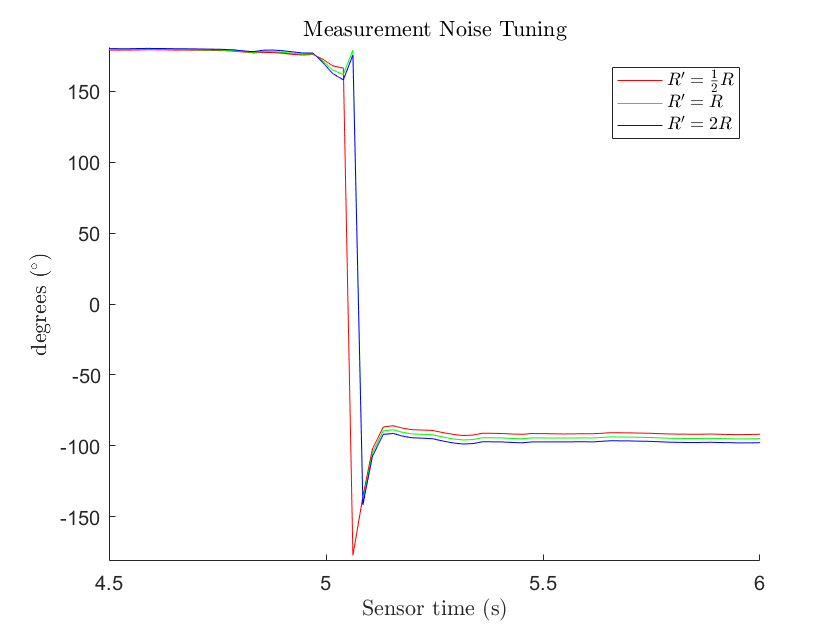
\includegraphics[width=0.6\textwidth]{OrientationRTuning}
	\end{center}
	\caption{Tuning the measurement noise parameter of the Kalman filter}
	\label{fig:computervis}
\end{figure}

Lower values of $R$ lead to a faster step response but more overshoot because the Kalman gain is high. Higher values of $R$ have a slower step response but less overshoot because the Kalman gain is lower. 

\subsubsection{Filter Performance}

The performance of the extended Kalman Filter model for the orientation is summarized in the charts in \ref{fig:kalmanerrorsummary}.

\begin{figure}[H]
    \begin{center}$
        \begin{array}{cc}
            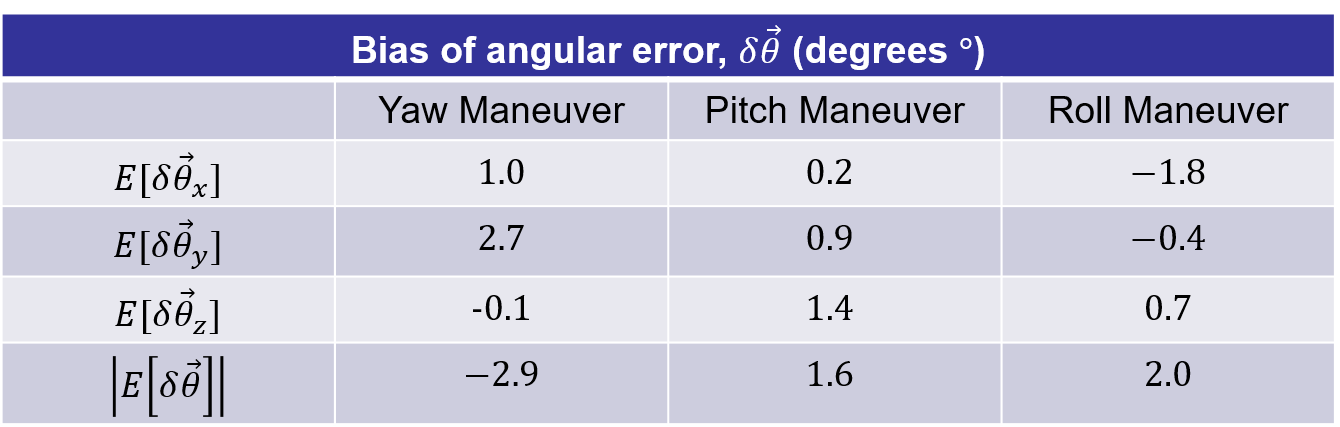
\includegraphics[width=0.5\textwidth]{KalmanBias} \\
            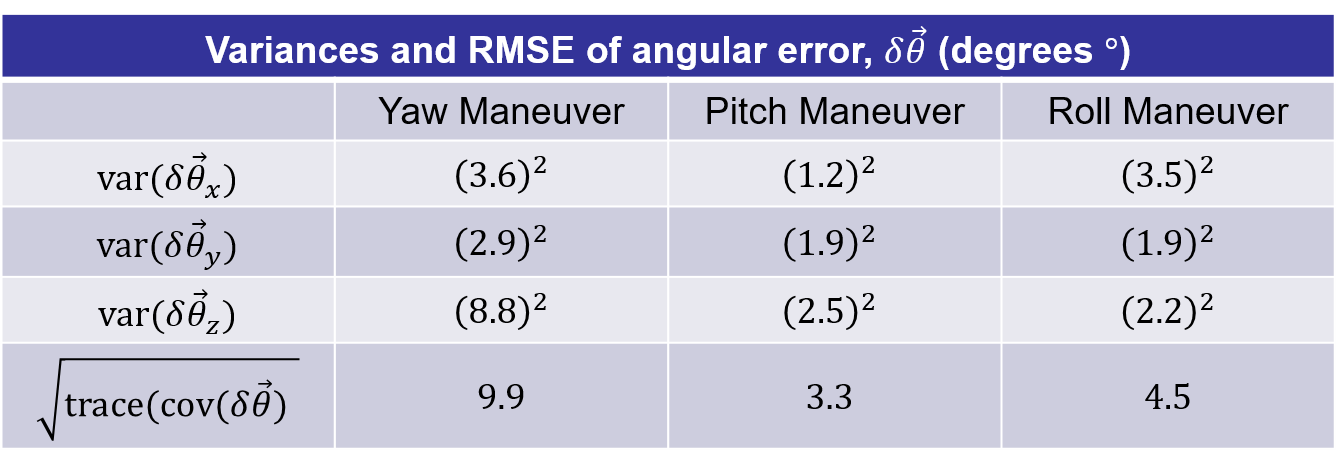
\includegraphics[width=0.5\textwidth]{KalmanVariance}
        \end{array}$
    \end{center}
    \caption{Kalman filter orientation tracking errors}
    \label{fig:kalmanerrorsummary}
\end{figure}

The comparison in the precision of these results to the TRIAD estimation algorithm is shown in \ref{fig:filtercomparison1}. 

\begin{figure}[H]
    \begin{center}$
        \begin{array}{cc}
            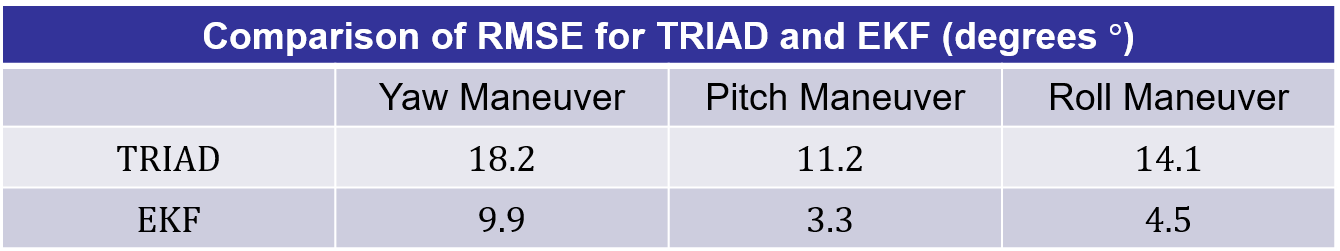
\includegraphics[width=0.5\textwidth]{FilterComparison}
        \end{array}$
    \end{center}
    \caption{Kalman filter and TRIAD root-mean-squared error comparison}
    \label{fig:kalmanerrorsummary}
\end{figure}

%%%%%%%%%%%%%%%%%%%%%%%%%%%%%%%%%%%%%%%%%%%%%%%%%%%%%%%%%%%%%%%%%%%%%%%%%%%%%%%
%% Position tracking
%%%%%%%%%%%%%%%%%%%%%%%%%%%%%%%%%%%%%%%%%%%%%%%%%%%%%%%%%%%%%%%%%%%%%%%%%%%%%%%

\section{Position Tracking}

%%%%%%%%%%%%%%%%%%%%%%%%%%%%%%%%%%%%%%%%%%%%%%%%%%%%%%%%%%%%%%%%%%%%%%%%%%%%%%%
%% Naive measurement model
\subsection{Measurement Model}

The following is a model of a single frame from the camera. In this frame, shown in image Figure \ref{fig:computervis} the red circular object represents the rear of the interaction tool. The spherical objecti of the rear of the interaction tool is called the tracking target. The width of the target along the $x$ dimension of the image is $s_{u}$. 

\medskip

\begin{figure}[H]
	\begin{center}
		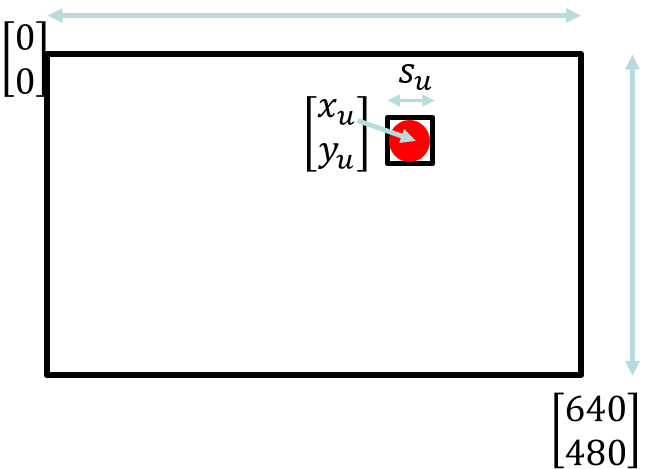
\includegraphics[width=0.8\textwidth]{computerVision}
	\end{center}
	\caption{Computer vision tracking model}
	\label{fig:computervis}
\end{figure}

\medskip

The midpoint of the target in the ideal undistorted image is $\pu = \mat{ x_u & y_u }^{T}$. The center of the undistorted image is $c_x$ in the x direction and $c_y$ in the y direction. The focal lengths in the x and y directions are $f_x$ and $f_y$, respectively. These parameters are found through the camera calibration routine, explained in detail below. The measurements of the center of the target and its width are related to the hidden state $\prpr = \mat{ x_s & y_s & z_s }^{T}$ in the following way: 

\[
    \y = h(\x)
        = \mat{x_u \\ y_u \\ s_{u} }
        = \mat{ \frac{f_x x_s}{z_s} + c_x \\ 
             \frac{f_y y_s}{z_s} + c_y \\ 
             \frac{s_c}{z_s \sqrt{\frac{1}{f_x^{2}} + \frac{1}{f_y^{2}}}}
           }
\]

These relationships are found through using a simple pin-hole camera model \cite{Tsai1987}.


\subsubsection{Camera Calibration}

The measurement model requires knowledge of the intrinsic camera parameters, $f_x, f_y, c_x, c_y$, and the radial and tangential distortion factors. There are two steps to translating a point from camera coordinates to image coordinates \cite{Tsai1987}. First, the pin-hole camera model shows how to find the ideal image coordinates of an object, $(\mathbf{x_u}, \mathbf{y_u})$ based on the position of the object in camera coordinates, $\prpr = (x, y, z)$: 

$$ \mathbf{x_u} = f_x \frac{x}{z} $$
$$ \mathbf{y_u} = f_y \frac{y}{z} $$

Second, the radial and tangential distortion relations show how the actual image coordinates, $(\mathbf{x_u}, \mathbf{y_u})$, relate to the image coordinates on the actual or distorted image plane, $(\mathbf{x_d}, \mathbf{y_d})$. The radial distortion correction equation is as follows: \\

$$ \mathbf{x_u} = x_d (1 + k_1 r^2 + k_2 r^4 + k_3 r^6) $$
$$ \mathbf{y_u} = y_d (1 + k_1 r^2 + k_2 r^4 + k_3 r^6) $$

and the tangential distortion equation is given by, 

$$ \mathbf{x_u} = x_d + (2 p_1 x y + p_2 (r^2 + 2x^2))$$
$$ \mathbf{y_u} = y_d + (p_1 (r^2 + 2y^2) + 2p_2 x y)$$

Thus, the five distortion parameters are summarized in a vector $D$: 

$$D = \mat{ k_1 & k_2 & p_1 p_2 & k_3 }$$

The calibration parameters are discovered by using an open source implementation provided by OpenCV. The camera collects a series of images that contain a checkerboard pattern. The calibration computes the transformation from the image coordinates of the checkerboard to its real world coordinates. The calibration images look like the ones in figure 1 below. 

\begin{figure}[H]
    \begin{center}$
        \begin{array}{cc}
            \includegraphics[width=0.2\textwidth]{image1} &
            \includegraphics[width=0.2\textwidth]{image2} \\
            \includegraphics[width=0.2\textwidth]{image3} &
            \includegraphics[width=0.2\textwidth]{image4} \\
        \end{array}$
    \end{center}
    \caption{Camera calibration routine}
    \label{fig:cameracalib}
\end{figure}

\subsubsection{Object Tracking}

The signal processing layer contains an object tracker to find the rear of the interaction tool in each frame. Since a robust estimate of the object size in each image is required, its edges must be estimated as exactly as possible. One simple way to estimate the edges of the spherical tracking target is to segment the tracking target from the background by using color. The color of the object is used determine which pixels belong to it and which to not. Additionally, the color-based object tracking must happen in real time. To meet the demands of real-time, color-based object tracking, the CamShift algorithm was chosen \cite{bradski1998}.

\subsubsection{Tool Maneuvers}

The possible maneuvers of the interaction tool are classified into two categories: maneuvers in the image plane and those in the depth dimension. For a user of the 3D Interaction Tool, side-to-side or up-and-down movements of the interaction tool map to motions in the image plane of the tracking camera, while movements of the tool towards and away from their body map to motions in the depth dimension. More precisely, the maneuvers in the image plane are movements of the interaction tool that occur perpendicular to the viewing angle of the camera. 

\medskip

The convention established for the purposes of testing is that the image plane is the yz-plane of the coordinate system and the depth dimension maps to the negative x-dimension. Maneuvers in the x-dimension encompass the movements of the tool towards and away from the tracking camera. Figure \ref{fig:imageplane} compares the actual motion of the interaction tool to the estimates made by the tracking system.

\begin{figure}[H]
    \begin{center}$
        \begin{array}{cc}
            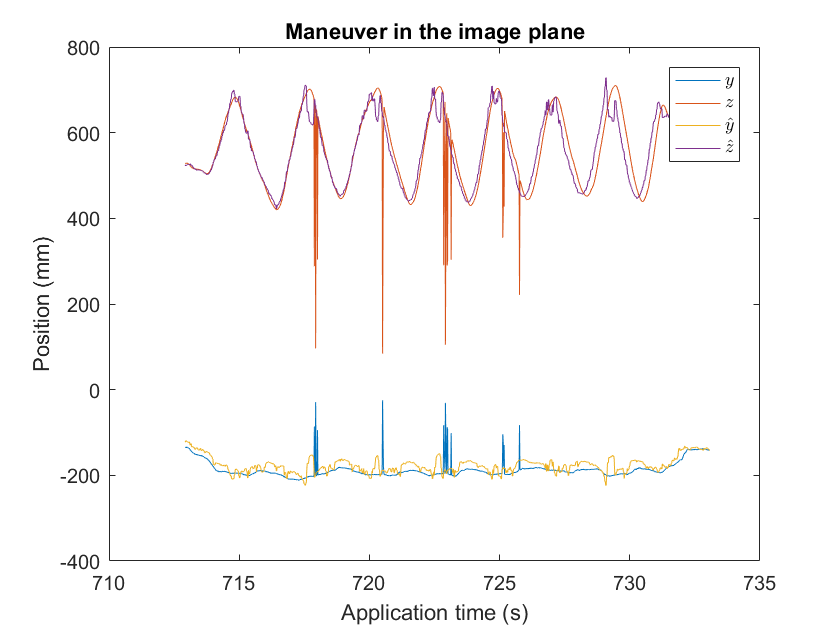
\includegraphics[width=0.5\textwidth]{ImagePlaneVertical} &
            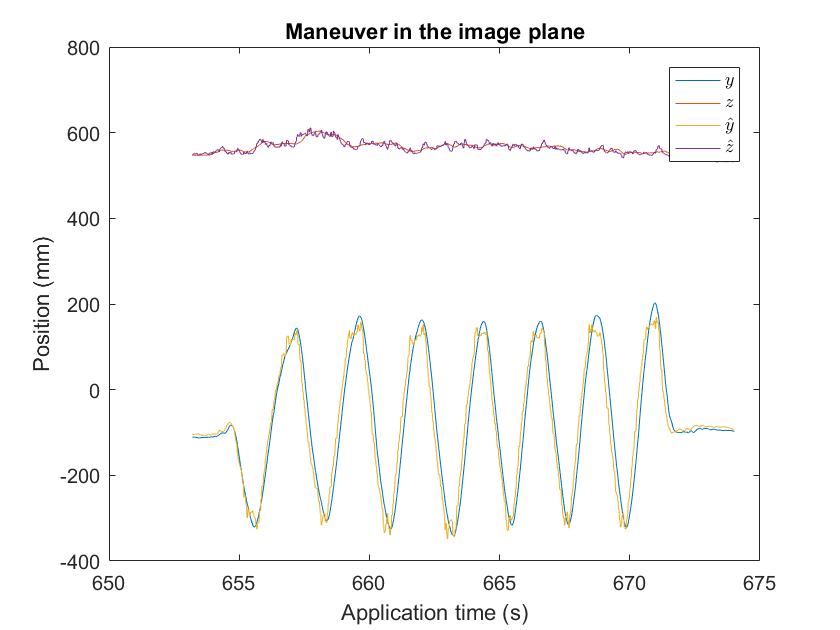
\includegraphics[width=0.5\textwidth]{ImagePlaneHorizontal} \\
        \end{array}$
    \end{center}
    \caption{Vertical and horizontal motion in the image plane}
    \label{fig:imageplane}
\end{figure}

In \ref{fig:imageplane}, the traces on the left correspond with vertical maneuvers of the tool and the traces on the right correspond to horizontal movements of the tool. In both graphs it is apparent that the tracking system is very accurate with low bias. The estimates of $\hat{y}$ and $\hat{z}$ map almost exactly to the true values.

\medskip

The second set of maneuvers are those in the depth dimension. Figure \ref{fig:depth} shows a trace of the actual depth $x$ and the estimated depth $\hat{x}$. 

\begin{figure}[H]
    \begin{center}$
        \begin{array}{cc}
            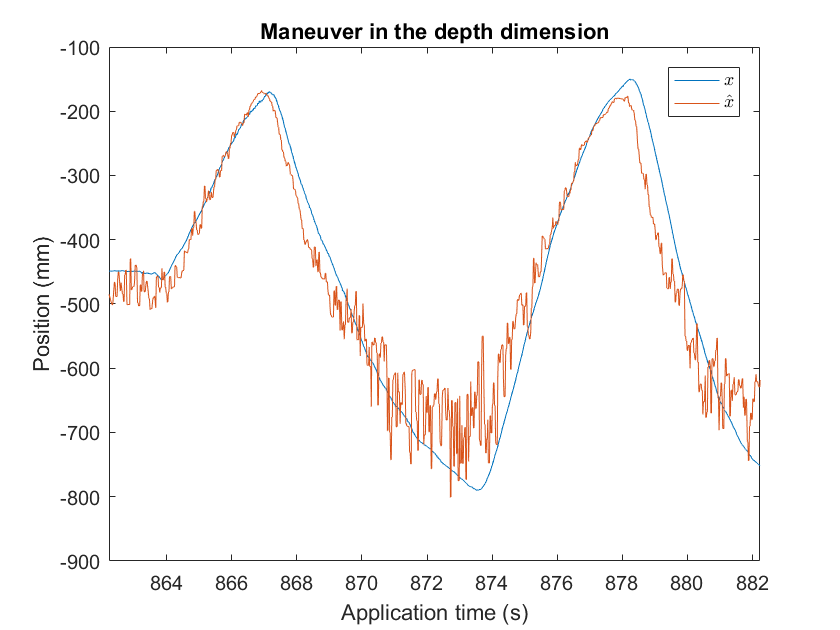
\includegraphics[width=0.8\textwidth]{DepthManeuver} &
        \end{array}$
    \end{center}
    \caption{Motion of the interaction tool in the depth dimension}
    \label{fig:depth}
\end{figure}

The natural conclusion from the traces in \ref{fig:depth} is that the depth tracking accuracy and precision depend on how far away the interaction tool is from the tracking camera.

\subsubsection{Error Analysis of Motion in the Image Plane}

The accuracy and precision of the tracking system depends on the direction of the tool maneuvers. This is evident from analyzing the covariance of the error in the $y$ and $z$ directions for vertical and horizontal maneuvers. Figure \ref{fig:yzerror} shows the error ellipse associated with motion in the image plane. On the left is the error ellispse associated with vertical motion and on the right is the error associated with horizontal motion. 

\begin{figure}[H]
    \begin{center}$
        \begin{array}{cc}
            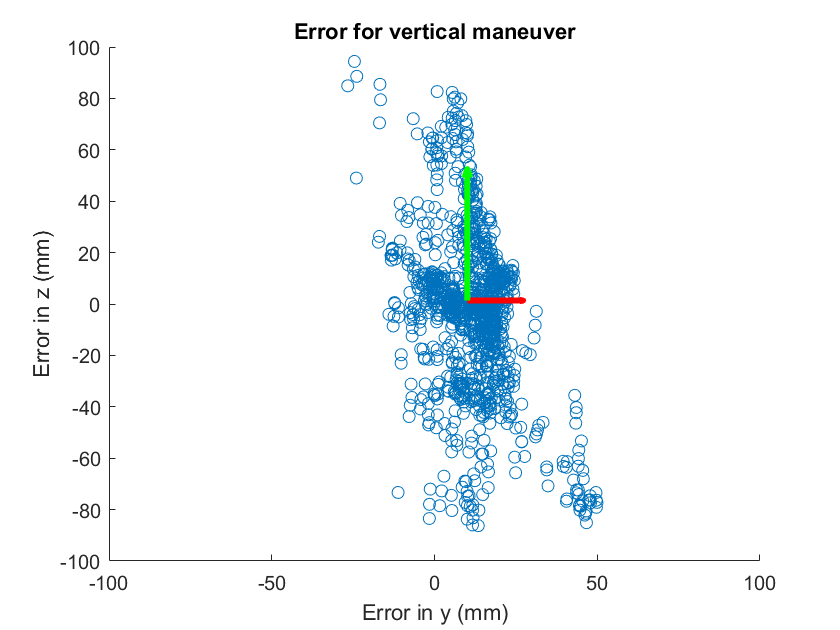
\includegraphics[width=0.5\textwidth]{ErrorElipseVertical} &
            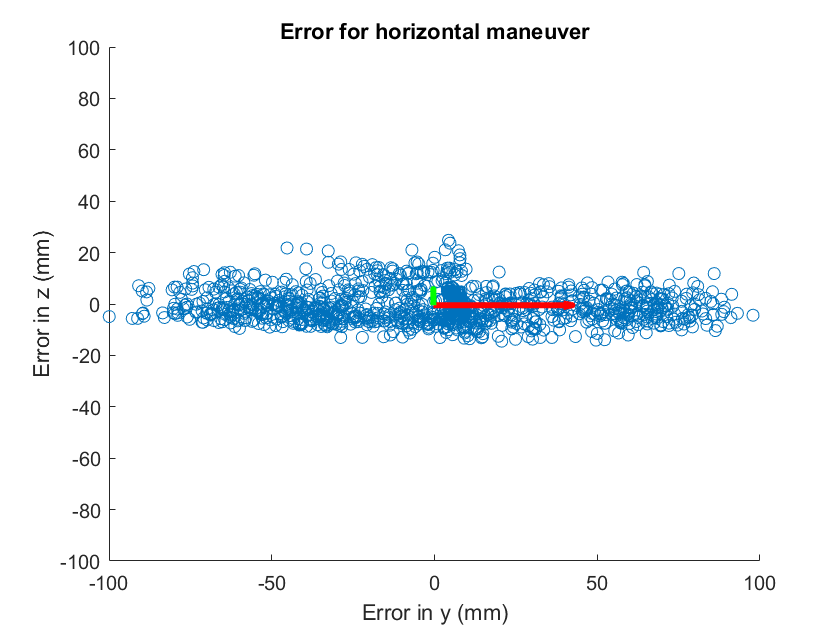
\includegraphics[width=0.5\textwidth]{ErrorElipseHorizontal} \\
        \end{array}$
    \end{center}
    \caption{Tool tracking errors in the yz-plane}
    \label{fig:yzerror}
\end{figure}

In \ref{fig:yzerror} two arrows are placed with their origins at the mean of the yz-error distribution and their length corresponding to the square root of the variance along the direction they point. It is clear from the magnitudes of these arrows that their is a breakdown of precision of the tracking system along the direction of motion for the 3D Interaction Tool.

\medskip

What explains the higher variance along the direction of motion for the interaction tool? There are essentially two sources of errror for tracking the target relative to the camera. First, there is error that comes from the camera calibration routine in the form of error of intrinsic parameters of the camera -- errors in $fx$, $fy$, for example. Second, there is error that comes from finding the centroid of the object in each image frame. Broadly, we could classify the calibration errors as systemic and the image processing errors as dynamic. Since the variance of the tool tracking increases in the direction of motion of the object, it is not likely that this error comes from a systemic problem with the calibration routine. Therefore, we can attribute the descrease in precision to error in the image segmentation routine. 

\medskip

Why does motion along a particular direction increase the error in the image segmentation? When the object is moving, its boundaries become blurred along the direction of motion in each frame. These blurred edges increase the uncertainty about the location of the object along the direction of motion. Therefore, when the object is moving along a particular direction, the uncertainty of its location in the direction of motion increases, but quickly drops again when the motion of the object halts.

\subsubsection{Error Analysis of Motion in the Depth Dimension}

The distribution of errors is larger for depth-tracking than tracking in the image plane. This result is displayed graphically in Figure \ref{fig:deptherror}. 

\begin{figure}[H]
    \begin{center}$
        \begin{array}{c}
            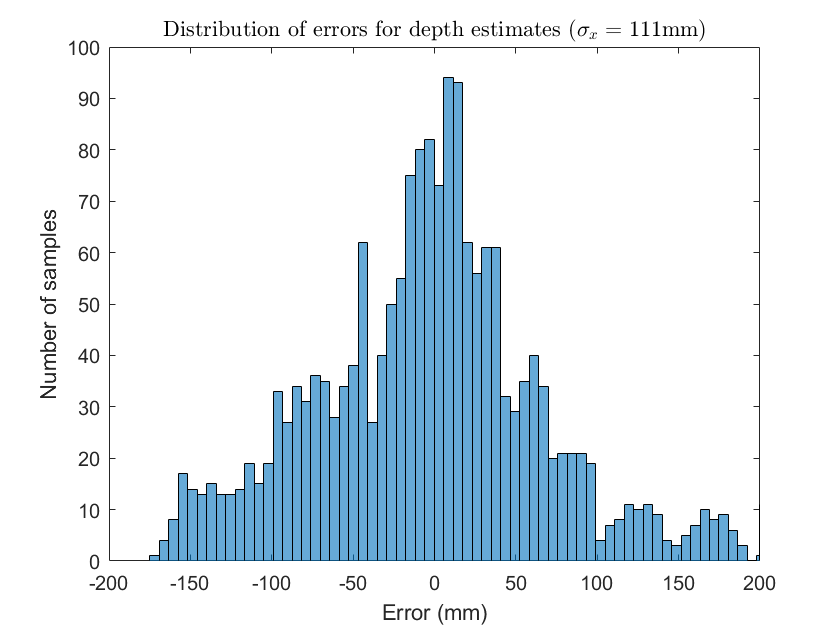
\includegraphics[width=0.8\textwidth]{ErrorHistDepth}
        \end{array}$
    \end{center}
    \caption{Distribution of depth-tracking errors}
    \label{fig:deptherror}
\end{figure}

While the bias of the tracking errors tends to zero, the variance is much larger than for the depth-tracking in the image plane.



%%%%%%%%%%%%%%%%%%%%%%%%%%%%%%%%%%%%%%%%%%%%%%%%%%%%%%%%%%%%%%%%%%%%%%%%%%%%%%%
%% Dynamic measurement model

\subsection{Dynamic Measurement Model}

Since the user's movement of the interaction tool is voluntary, no assumptions can be made about its overall trajectory. However, human-motion objeys minimum-jerk constraints \cite{flash1985}. Since the jerk of the tool's motion is small, it can be modelled as a white-noise process. The dynamical model for the tool's motion along the $x$ axis is estimated by the discrete time state-space model

$$ \vec{x}_{k+1} = \mat{1 & \Delta t \\ 0 & 1} \mat{x \\ \xd} + \mat{0 \\ \Delta t} \xdd  + \mat{0 \\ 1} w_k $$

where $w_k$ is the jerk. Additionally, the motion of the tool is assumed to be coordinate uncoupled, since the user is free to move the tool in any direction. Therefore this same model can be extended to motion along the $y$ and $z$ axes as well.


%%%%%%%%%%%%%%%%%%%%%%%%%%%%%%%%%%%%%%%%%%%%%%%%%%%%%%%%%%%%%%%%%%%%%%%%%%%%%%%
%% Performance Analysis
%%%%%%%%%%%%%%%%%%%%%%%%%%%%%%%%%%%%%%%%%%%%%%%%%%%%%%%%%%%%%%%%%%%%%%%%%%%%%%%
\section{Performance Analysis}

This section summarizes the performance of the tracking system implementation according to the performance design goals.

\subsection{Robustness}

No quantitative metrics were made for the robustness of the tracking system. In order to make the object tracking system workable, so that the CamShift algorithm could find the position of the tool rear in each frame, a Kalman filter was implemented to predict the next location of the bounding box of the interaction tool, following the method of \cite{camshiftkalman}.

\subsection{Latency Calculation}

The latency calculation goes as follows. We differentiate the VICON reference position signal to find a reference acceleration signal. Second, we compute the time shift $\Delta s$ between the the acceleration readings from the accelerometer and those from the VICON tracking system. Third, we calculate the time shift $\Delta e$ between the position estimates of the filter and the VICON reference clock. Finally, we find the latency, $\Delta t$ by taking the difference between the times of the sensor measurements and the position estimates. The autocorrelation graphs are shown in Figure \ref{fig:autocorr}

\begin{figure}[H]
    \begin{center}$
        \begin{array}{cc}
            \includegraphics[width=0.5\textwidth]{AutoCorr}
        \end{array}$
    \end{center}
    \caption{Autocorrelations for latency calculation}
    \label{fig:autocorr}
\end{figure}

The result of the latency calculation shows an overall latency of $22$ms, including latency in the system itself. This latency corresponds to the frame update rate of the camera.


\subsection{Estimation Error}

Given the tool model $ \pfe = \pre + \ple $, the overall error covariance $\Ppf$ is a function of the error due to the position estimation and the error to the orientation estimation. Since the estimation of $\pr$ and $\pl$ occur independently, it is reasonable to assume that the errors in the estimation of these vectors is not correlated. Thus, the covariances of the errors for these two vectors simply add to yield the covariance of the error for the tool front: 

\begin{equation} \label{eq:Ppf}
    \Ppf =  \Ppr + \Ppl
\end{equation}

\subsection{Covariance Transformations}

Here are three properties of covariance transformations, useful for analysing the performance of the tracking system as a whole: 

\medskip

(1) Given two independent random variables $X$, $Y$, and their sum $Z = X + Y$ how does the covariance of $Z$ $\Sigma_Z$ relate to the covariances $\Sigma_X$ and $\Sigma_Y$ of $X$ and $Y$, respectively? In this case the covariances simply sum so that 

$$ \Sigma_Z = \Sigma_X + \Sigma_Y $$

\medskip

(2) Given two random variables $X$ and $Y$ related by the linear operator $T$ so that $ Y = T X $ how does the covariance of $Y$ relate to the covariance of $X$?  If $\Sigma_X$ is the covariance of $X$ and $\Sigma_Y$ is the covariance of $Y$, then 

$$ \Sigma_Y = T \Sigma_X T^T $$  

\medskip

(3) Given two random variables $X$ and $Y$, and the non-linear relationship that $Y = f(X)$, how does the covariance of $Y$ change with the covariance of $X$? As a first-order approximation, the randomness of $Y$ can be approximated as a linear function of $X$ \cite{haralick1996}: 

\begin{equation} \label{eq:firstorderdev}
    Y - \mu_Y = T (X - \mu_X)
\end{equation}

Now, given the linear relationship, $Y - \mu_Y = T (X - \mu_X) $, the covariance of $Y$ is related to the covariance of $X$ by 

$$ \Sigma_Y = T \Sigma_X T^{T} $$

using property (2) of the covariance transformation under a linear operator.

\subsection{Estimation Error for $\ple$: Finding position error due to orientation error}

How do errors in the orientation estimation lead to errors the tool position estimation? In the tool model, the position of the front of the tool is estimated from three pieces of information: the position of the rear of the tool $\pr$, the orientation of the tool $\At$, and the tool length in body coordinates $\plpr$. This relationship is described by the equation 

$$ \pf = \pr + \pl = \pr + \At^{T} \plpr $$ 

There is no error in the measurement of $\plpr$; that is a well known parameter of the interaction tool. The error in $\pl$ comes from the estimation of the rotation matrix from body coordinates to world coordinates. 

\medskip

The attitude matrix $\At$ is parameterized by the quaternion $\qt$ estimated from the EKF so that $\pl = \At(\qt)^{T} \plpr$. This expression is helpful because it describes the tool span vector $\pl$ as a function of $\qt$. The relationship between $\pl$ and $\qt$ must be linearlized in order to understand how errors in the estimation of $\qt$ translate to errors in $\pl$. 

\medskip

Let the small deviations in the orientaiton be represented by the error quaternion $\dq$ so that $\pl = \A(\dq) \At(\qt)^{T} \plpr$, where $\A(\dq)$ is the attitude matrix parameterized by the orientation error. Then, the goal here is to linearize the relationship between $\pl$ and $\dq$, and to accomplish we find the matrix first-order derivative of $\pl$ with respect to the three dimensional representation of the error quaternion $\dqvec$: 

$$ \deldq = \ddq \A(\dq) \At(\qt)^T \plpr $$

Now simplify $\A(\dq)$ using the assumptions that $\dqw \approx 1$ and $|\dqvec| \approx 0$, both of which will be true for small errors:

$$ \A(\dq) = (|\dqw|^2 - |\dqvec|) I_{3x3} + 2 \dqvec \dqvec^T - 2\dqw\crossmat{\dqvec}  = I_{3x3} - 2\crossmat{\dqvec} $$

Pplugging in this expression for $\A(\dq)$: 

$$ \deldq = \ddq (I_{3x3} - 2\crossmat{\dqvec}) \At(\qt)^T \plpr $$

Note that $\At(\qt)^T \plpr$ is a constant vector -- in fact it is simply the estimate for $\pl$! 

$$ \deldq = \ddq( I_{3x3} \pl - 2 \crossmat{\dqvec} \pl )  = -2 \ddq \crossmat{\dqvec} \pl $$

The quantity $\crossmat{\dqvec} \pl$ is simply $\dqvec \times \pl = -\pl \times \dqvec$. Therefore, 

$$ \deldq = -2 \ddq (-\pl \times \dqvec) = 2 \crossmat{\pl} \ddq \dqvec = 2 \crossmat{\pl} $$

Now we can write deviations in $\pl$ as a linear function of the quaternion error or angular error ( $\dqvec = \frac{1}{2} \dtvec$ ): 

$$ \delta\pl = 2 \crossmat{ \At(\qt)^T \plpr } \dqvec  =  \crossmat{ \At(\qt)^T \plpr } \dtvec $$

This is written in the form of Equation \ref{eq:firstorderdev}. Thus, if $\Ptt$ is the covariance of the estimation of the tool's orientation, then the covariance $\Ppl$ of $\pl$ is

\begin{equation} \label{eq:plcovariance}
    \Ppl = \crossmat{ \At(\qt)^T \plpr } \Ptt \crossmat{ \At(\qt)^T \plpr }^T 
        = \At(\qt)^T \crossmat{\plpr} \Ptt \crossmat{\plpr}^T \At(\qt)
\end{equation}

\subsection{Overall performance} 

The trace of the covariance matrices are invariant to linear transformations, thus we can derive the expression that 

$$ \tr(\Ppf) = \tr(\Ppr) + \tr(\Ppl) = \tr(\Pprpr) + l^2 \tr(\Ptt) $$

Equivalently, 

$$ \mse(\pf) = \mse(\prpr) + l^2 \mse(\hat{\vec{\theta})}) $$

Thus the overall error of the estimation of the position of the front of the tool in world coordinates depends on the position estimation error and the square of the length of the tool times the orientation estimation error. Using the error estimates derived in the sections on position and orientation tracking, this result is summarized in Figure \ref{fig:overallerror}

\begin{figure}[H]
    \begin{center}$
        \begin{array}{cc}
            \includegraphics[width=0.5\textwidth]{OverallPerformance}
        \end{array}$
    \end{center}
    \caption{Overall tracking error given position and orientation tracking errors}
    \label{fig:overallerror}
\end{figure}

This chart illuminates the following result: the position tracking errors dominate, with root-mean-squared error of only $1$cm coming from the errors in the orientation tracking.


% Covariance equations
% $$ \Pprpr = \Pprpr + \crossmat{\pspr} \Pacpr \crossmat{\pspr}^T $$
% $$ \Ppr = \Acinv ( \Pprpr + \crossmat{\pspr} \Pacpr \crossmat{\pspr}^T ) (\Acinv)^T + \Ppc $$
% $$ \Ppf = \Ppr + \Atinv \crossmat{\pl} \Patpr \crossmat{\pl}^T (\Atinv)^T $$
% $$ \Ppfpr = \Ad ( \Ppf + \Ppd ) \Ad{^T} $$
% $$ \Ppfpr = \Pprpr + \crossmat{\pspr} \Pacpr \crossmat{\pspr}^T + \Atpr \crossmat{\pl} \Patpr \crossmat{\pl}^T (\Atpr)^T + 2\Ad\Ppd\Ad{^T} $$

%%%%%%%%%%%%%%%%%%%%%%%%%%%%%%%%%%%%%%%%%%%%%%%%%%%%%%%%%%%%%%%%%%%%%%%%%%%%%%%
%% Conclusion
%%%%%%%%%%%%%%%%%%%%%%%%%%%%%%%%%%%%%%%%%%%%%%%%%%%%%%%%%%%%%%%%%%%%%%%%%%%%%%%
\section{Conclusion}

Revisiting the design objectives in \ref{fig:performance}, the table in Figure \ref{fig:summary1} captures the progress made on the performance of the tracking system. In green are those specifications that were achieved, and in orange are the specifications towards with progress was made. 

\begin{figure}[H]
    \begin{center}
		\includegraphics[width=1\textwidth]{PerformanceRevisited}
    \end{center}
    \caption{Performance design goals, revisited}
    \label{fig:summary1}
\end{figure}

The specifications for the latency and orientation error were achieved so that the lag of the system is not noticable and the estimation errors are imperceptible to the user. The root-mean-squared error for the position estimates was about twice that which was specified. These position errors were largely due to errors in the depth dimension of the tracking camera and errors due to tool velocity. 

\begin{figure}[H]
    \begin{center}
		\includegraphics[width=1\textwidth]{UsabilityRevisited}
    \end{center}
    \caption{Performance design goals, revisited}
    \label{fig:summary2}
\end{figure}

Figure \ref{fig:summary2} revisits the design objectives in \ref{fig:usability}. Portability and form factor requirements were met. The cost specification is easy to meet in future prototypes. The sensors used for the intial prototype were particularly expensive because they came with on-board filtering that was useful for prototyping. However, now that the tracking algorithms are implemented, lower-part costs could be purchased for any future prototypes. 

\medskip

The tracking volume objective can be met by increasing the field of view of the camera. Some experiments were done in this configuration, but they introduce a large bias into the position estimates due to errors in the calibration of the distortion parameters associated with widening the field of view of the lens. 



%%%%%%%%%%%%%%%%%%%%%%%%%%%%%%%%%%%%%%%%%%%%%%%%%%%%%%%%%%%%%%%%%%%%%%%%%%%%%%%
%% Future Work
%%%%%%%%%%%%%%%%%%%%%%%%%%%%%%%%%%%%%%%%%%%%%%%%%%%%%%%%%%%%%%%%%%%%%%%%%%%%%%%
\section{Future Work}

% \end{multicols}

\bibliographystyle{ieeetr}
\bibliography{references}

\end{flushleft}
\end{document} 
